\documentclass[11pt]{article}

\usepackage[a4paper,margin=1in]{geometry}
\usepackage[T1]{fontenc}
\usepackage[utf8]{inputenc}
\usepackage{lmodern}
\usepackage{microtype}
\usepackage{amsmath,amssymb}
\usepackage{booktabs}
\usepackage{tabularx}
\usepackage{graphicx}
\usepackage{siunitx}
\usepackage{caption}
\usepackage{subcaption}
\usepackage{enumitem}
\usepackage{xcolor}
\usepackage{hyperref}
\usepackage[nameinlink,noabbrev]{cleveref}

\graphicspath{{figures/}}
\sisetup{separate-uncertainty=true}
\setlength{\parindent}{0pt}
\setlength{\parskip}{0.55em}

\hypersetup{
  colorlinks=true,
  linkcolor=blue!55!black,
  citecolor=blue!55!black,
  urlcolor=blue!55!black,
  pdftitle={SiPM Operating-Point Calibration for the gLOWCOST Detector},
  pdfauthor={Tharindu Hettiarachchi}
}

\newcommand{\vbr}{V_{\mathrm{br}}}
\newcommand{\vbias}{V_{\mathrm{bias}}}
\newcommand{\vov}{V_{\mathrm{OV}}}
\newcommand{\pe}{\mathrm{p.e.}}
\newcolumntype{Y}{>{\raggedright\arraybackslash}X}

\title{SiPM Operating-Point Calibration\\
for the gLOWCOST Detector}
\author{Tharindu Hettiarachchi\\
Department of Physics and Astronomy, Georgia State University}
\date{September 2026}

\begin{document}

\maketitle

\begin{abstract}
The gLOWCOST detector uses plastic scintillator tiles, wavelength-shifting fibres, and silicon photomultipliers (SiPMs) to detect charged particles. Stable operation requires an SiPM bias that is high enough to detect scintillation light but not so high that dark counts, correlated avalanches, or readout saturation dominate. This work develops and tests a waveform-based method for measuring the breakdown voltage of Hamamatsu S13360-2050VE SiPMs through the existing gLOWCOST analogue readout. Dark-pulse waveforms were recorded with a PicoScope, corrected event by event for baseline offset, and integrated in a peak-aligned time gate. The spacing between neighboring photoelectron populations was used as a relative gain measurement and extrapolated linearly to zero spacing.

For the original SiPM pair, the internally determined breakdown voltages at \SI{20}{\degreeCelsius} were \SI{50.637(37)}{\volt} and \SI{51.988(103)}{\volt}. A later pair, physically marked Triangle and Star, was measured in two complete scans after a channel-dependent trigger problem was identified. Their weighted results near \SI{20.4}{\degreeCelsius} were \SI{50.512(83)}{\volt} and \SI{50.574(67)}{\volt}. The difference, \SI{0.062(106)}{\volt}, is not statistically significant. These uncertainties describe waveform analysis and repeatability; they do not yet include the full absolute calibration uncertainty of the MAX1932 and DAC bias system.

The study also establishes an EPIC-tile coincidence method for measuring the full response of GSU gLOWCOST tiles. This zero-event measurement is intended to test whether channels operated at equal overvoltage have equal practical detection efficiency. The current scintillator data are treated as method development rather than a completed photon-detection-efficiency measurement.
\end{abstract}

\tableofcontents
\newpage

\section{Introduction}

The gLOWCOST detector is being developed as a compact and inexpensive charged-particle detector. A particle crossing a plastic scintillator deposits energy and produces optical photons. A wavelength-shifting fibre collects part of this light and transports it to a silicon photomultiplier. The SiPM converts the light into a fast electrical pulse, which is amplified, compared with a threshold, and counted by an FPGA.

The operating voltage is one of the most important detector settings. An SiPM must be biased above its breakdown voltage, but the breakdown voltage is not identical for every device and changes with temperature. Raising the voltage increases the charge produced by one fired microcell and generally increases photon-detection efficiency. It also increases dark-count rate, optical crosstalk, and afterpulsing \cite{klanner2019,hamamatsuTechnical}. The best setting is therefore a measured operating point, not simply the highest allowed voltage.

This study began with a practical question: can the existing gLOWCOST readout be used to calibrate each SiPM without adding a separate charge-sensitive instrument? The work developed through several stages. Early manual waveform recordings showed photoelectron structure but also exposed problems with baseline treatment, trigger selection, and channel identity. The acquisition was then automated, the pulse-area method was made more robust, complete scans were repeated, and channel swaps were used to distinguish SiPM behavior from readout-path behavior.

The objectives were:

\begin{enumerate}[leftmargin=*]
  \item resolve photoelectron populations using the amplified analogue waveform;
  \item determine the response corresponding to one additional fired microcell;
  \item measure breakdown voltage from the gain-related spacing;
  \item test repeatability and sensitivity to trigger conditions;
  \item set provisional equal-overvoltage operating points; and
  \item prepare an independent particle-trigger measurement of full-chain efficiency.
\end{enumerate}

The last objective is important. Equal overvoltage is a useful starting condition, but it does not prove equal photon sensitivity. The scintillator, fibre, optical coupling, SiPM, amplifier, and software threshold all contribute to the response seen in the final detector.

\section{Detector and Readout}

\subsection{SiPM}

The devices studied were Hamamatsu S13360-2050VE MPPCs. The series datasheet gives a $\SI{2}{\milli\metre}\times\SI{2}{\milli\metre}$ photosensitive area, \SI{50}{\micro\metre} pixel pitch, 1584 pixels, a typical breakdown voltage near \SI{53}{\volt}, and a typical gain of approximately $1.7\times10^6$ under the stated manufacturer conditions \cite{hamamatsuDatasheet}. These are typical series values. They do not replace a measurement of the individual device installed in a detector.

An SiPM contains many microcells operated in Geiger mode. One carrier initiating an avalanche produces the charge of one fired cell. More than one fired cell produces a larger pulse. Repeated dark pulses can therefore form approximately equally spaced populations corresponding to one, two, three, or more fired cells.

\subsection{gLOWCOST analogue path}

The waveform was measured after the gLOWCOST analogue amplifier and before the comparator. The recorded signal therefore includes the SiPM response, the coupling network, the amplifier, cable and probe effects, and the PicoScope response. The comparator and FPGA are used during normal counting, but they were not used to measure the photoelectron spacing.

The non-inverting amplifier has a nominal gain of 101. This large gain makes single-cell structure visible on the scope, but it also means that saturation and bandwidth must be checked. A stable p.e. spacing measures the complete analogue-chain response to one additional fired cell. It is not automatically the absolute SiPM charge in coulombs.

\begin{figure}[htbp]
  \centering
  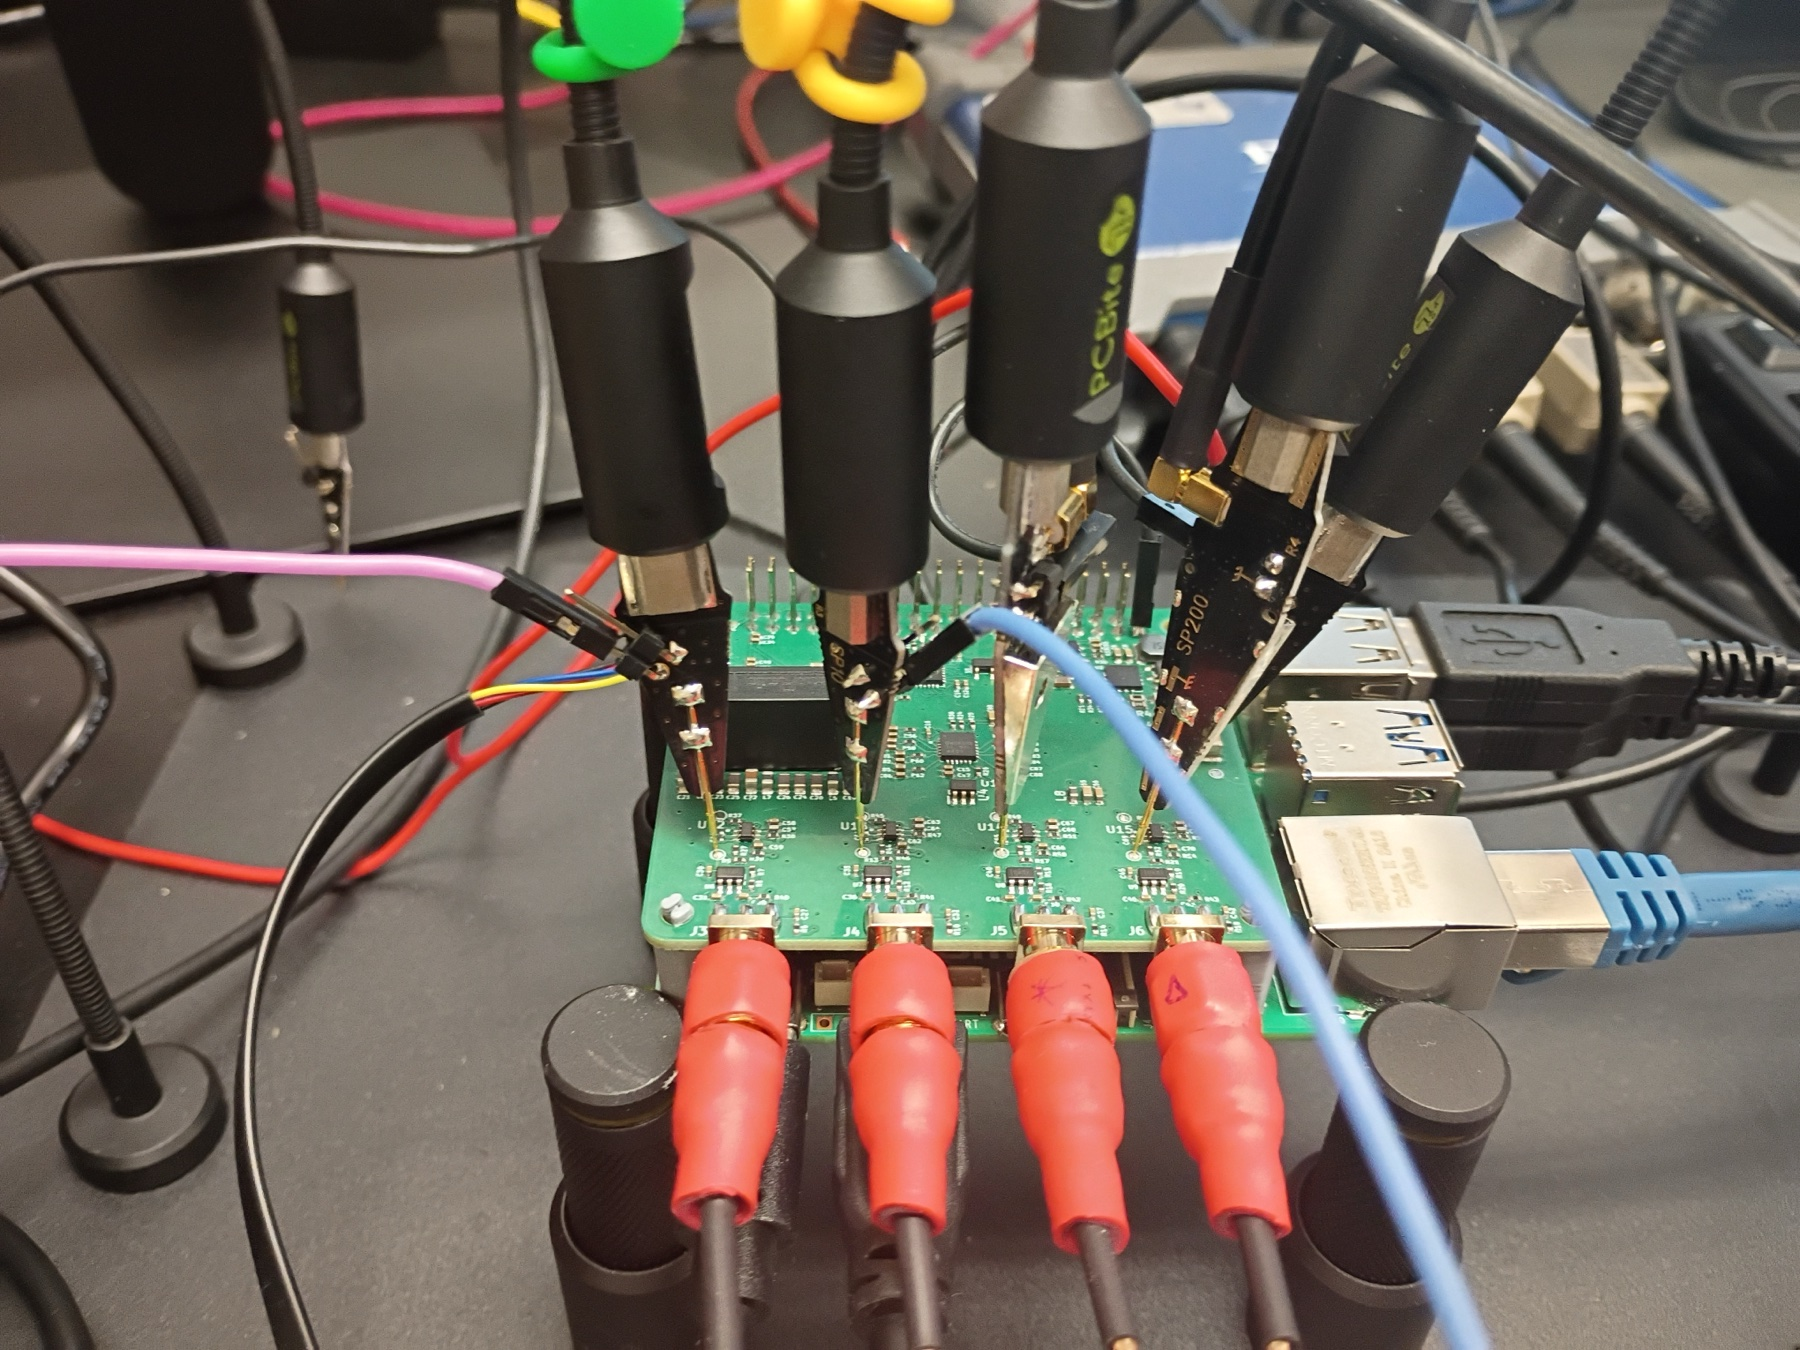
\includegraphics[width=0.88\linewidth]{readout-board.jpg}
  \caption{The four-channel gLOWCOST readout connected to the PicoScope. The analogue outputs were measured before the comparator.}
  \label{fig:readout-board}
\end{figure}

\subsection{Bias generation}

The detector uses a common high-side voltage from a MAX1932 circuit and an independently adjustable low-side voltage from a channel DAC. The effective SiPM bias is

\begin{equation}
  \vbias = V_{\mathrm{high}}-V_{\mathrm{low}}.
  \label{eq:effective-bias}
\end{equation}

The MAX1932 interface is write-only in the present hardware. A control code can be converted into a predicted voltage using a calibration relation, but this is not a live measurement at the SiPM terminals. The channel DAC also has a calibrated code-to-voltage relation. Their difference was used for the bias axis in this study.

Temperature compensation was disabled during controlled breakdown-voltage scans so that the voltage did not move while one point was recorded. Temperature was logged and, where stated, bias values were normalized using the provisional manufacturer coefficient of \SI{54}{\milli\volt\per\degreeCelsius}.

\subsection{Waveform instrumentation}

The main measurements used a PicoScope 3406B with 10:1 passive probes. The primary automated scans used a \SI{1}{\nano\second} sample interval and 10,000 waveforms at each voltage point. The acquisition configuration recorded probe ratio, range, coupling, trigger, time window, channel mapping, temperature, and bias commands.

The 10:1 correction is essential. Applying it twice would make the apparent signal ten times too large; omitting it would make the result ten times too small. The correction was therefore treated as part of the acquisition metadata rather than an informal plotting adjustment.

\section{Measurement Principle}

\subsection{Breakdown voltage and overvoltage}

The operating quantity is the overvoltage,

\begin{equation}
  \vov = \vbias-\vbr,
  \label{eq:overvoltage}
\end{equation}

where $\vbr$ is the breakdown voltage. Above breakdown, the avalanche charge from one microcell is approximately proportional to overvoltage over a useful operating interval. If the analogue readout remains linear, the spacing between neighboring photoelectron populations follows the same behavior,

\begin{equation}
  \Delta Q = m(\vbias-\vbr)=m\vbias+b,
  \label{eq:gain-line}
\end{equation}

where $\Delta Q$ is the measured pulse-area spacing and $m$ includes the SiPM cell capacitance and the readout conversion. The breakdown voltage is the x-intercept,

\begin{equation}
  \vbr=-\frac{b}{m}.
  \label{eq:vbr}
\end{equation}

This does not mean that a visible waveform is measured at zero amplitude below breakdown. The line is fitted to resolved photoelectron spacing above breakdown and extrapolated to the point where the gain-related spacing becomes zero. This use of gain extrapolation is established in SiPM characterization \cite{chmill2017,klanner2019}.

\subsection{Why pulse area was used}

Peak height is intuitive, but it depends on pulse width, sampling phase, ringing, and clipping. The primary observable in the final method was a peak-aligned integral,

\begin{equation}
  Q_{\mathrm{proxy}} = \int_{t_{\mathrm{peak}}-20\,\mathrm{ns}}^{t_{\mathrm{peak}}+200\,\mathrm{ns}}
  v(t)\,dt.
  \label{eq:pulse-area}
\end{equation}

Its unit is \si{\milli\volt\nano\second}. It is proportional to charge after the analogue chain, but it is called a charge proxy because the transfer impedance and full frequency response have not yet been calibrated. Peak height was retained as an independent cross-check.

\begin{figure}[htbp]
  \centering
  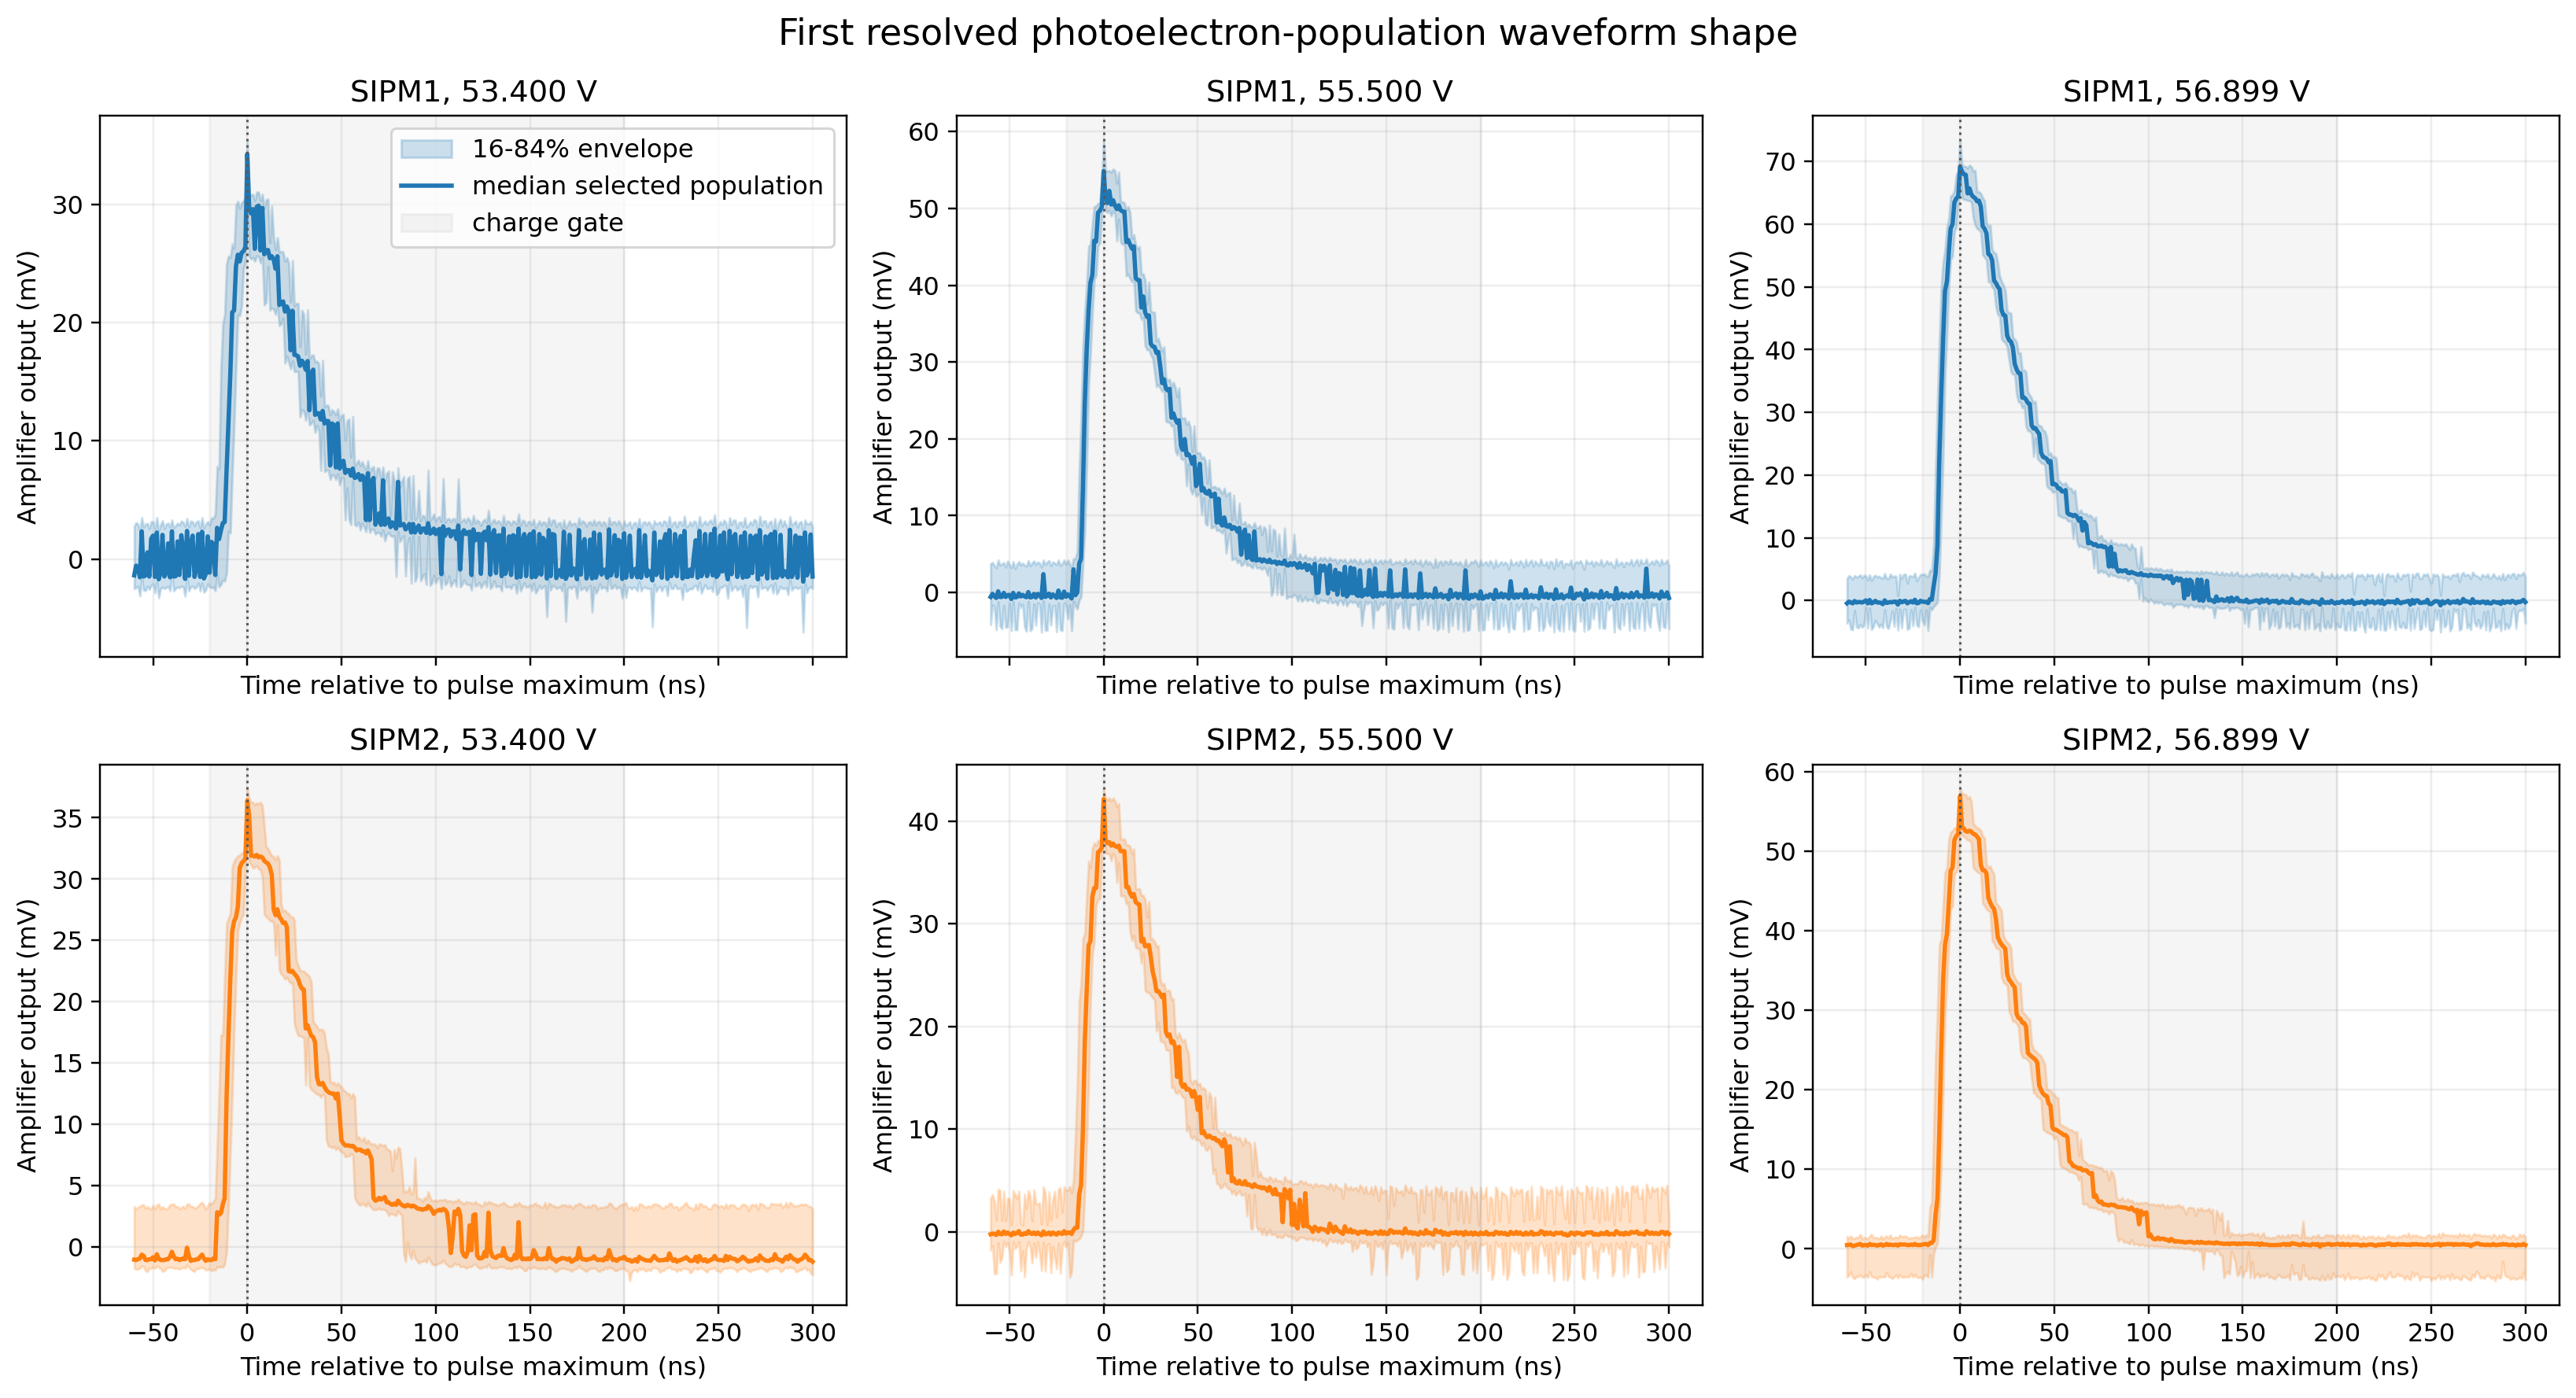
\includegraphics[width=0.92\linewidth]{single-pe-waveforms.png}
  \caption{Representative baseline-subtracted single-photoelectron waveform shapes used to define the prompt pulse region.}
  \label{fig:single-pe-waveforms}
\end{figure}

\section{Experimental Procedure}

\subsection{Dark-pulse scans}

The SiPM was light blocked. Thermal carriers still initiate avalanches, and optical crosstalk can make more than one microcell fire. These events provide the p.e. populations without an external light source.

For each bias point, the voltage was set, the hardware was allowed to settle, temperature was recorded, and the requested waveforms were saved. Each SiPM triggered on its own waveform. The automated sequence also recorded the final hardware state and was designed to turn off the high voltage after completion or failure.

An independent HV-off acquisition measured the electronic pedestal. The pedestal is the zero-avalanche response; it is not necessarily the first peak in a self-triggered dark-pulse histogram. The pedestal location and width were used to constrain the zero-p.e. population in the spectrum model.

\subsection{Channel mapping and swaps}

Physical SiPM labels, PCB channels, and scope channels were recorded separately. This was necessary because connections were deliberately exchanged during diagnosis. A result was assigned to a physical SiPM only when the mapping was known.

Two physical groups appear in the study:

\begin{table}[htbp]
  \centering
  \caption{SiPM groups used during the development of the method.}
  \label{tab:device-groups}
  \begin{tabularx}{0.96\linewidth}{l l Y}
    \toprule
    Group & Device labels & Main purpose \\
    \midrule
    Original pair & SIPM1, SIPM2 & Method development and repeated scans \\
    Later pair & SiPM 1 (Triangle), SiPM 2 (Star) & Channel diagnosis and clean repeats \\
    \bottomrule
  \end{tabularx}
\end{table}

The numerical results from these groups are not combined because they are different physical devices.

\subsection{Trigger study on PCB CH3}

The first measurements through PCB CH3 had very low acceptance at a \SI{15}{\milli\volt} PicoScope trigger. Swapping scope inputs did not move the behavior; it remained with the PCB path. A dedicated trigger scan at an effective bias of \SI{56.401}{\volt} found a sharp transition between \SI{15}{\milli\volt} and \SI{25}{\milli\volt}. Acceptance increased from 1.62\% to 99.82\%, while the extracted p.e. spacing remained stable from 20 to \SI{45}{\milli\volt}. A \SI{25}{\milli\volt} acquisition trigger was therefore used for the clean Triangle/Star scans.

This threshold was a PicoScope acquisition setting. It was not the comparator threshold used for normal detector counting, and it did not remove the underlying CH3 feature from the electronics.

\begin{figure}[htbp]
  \centering
  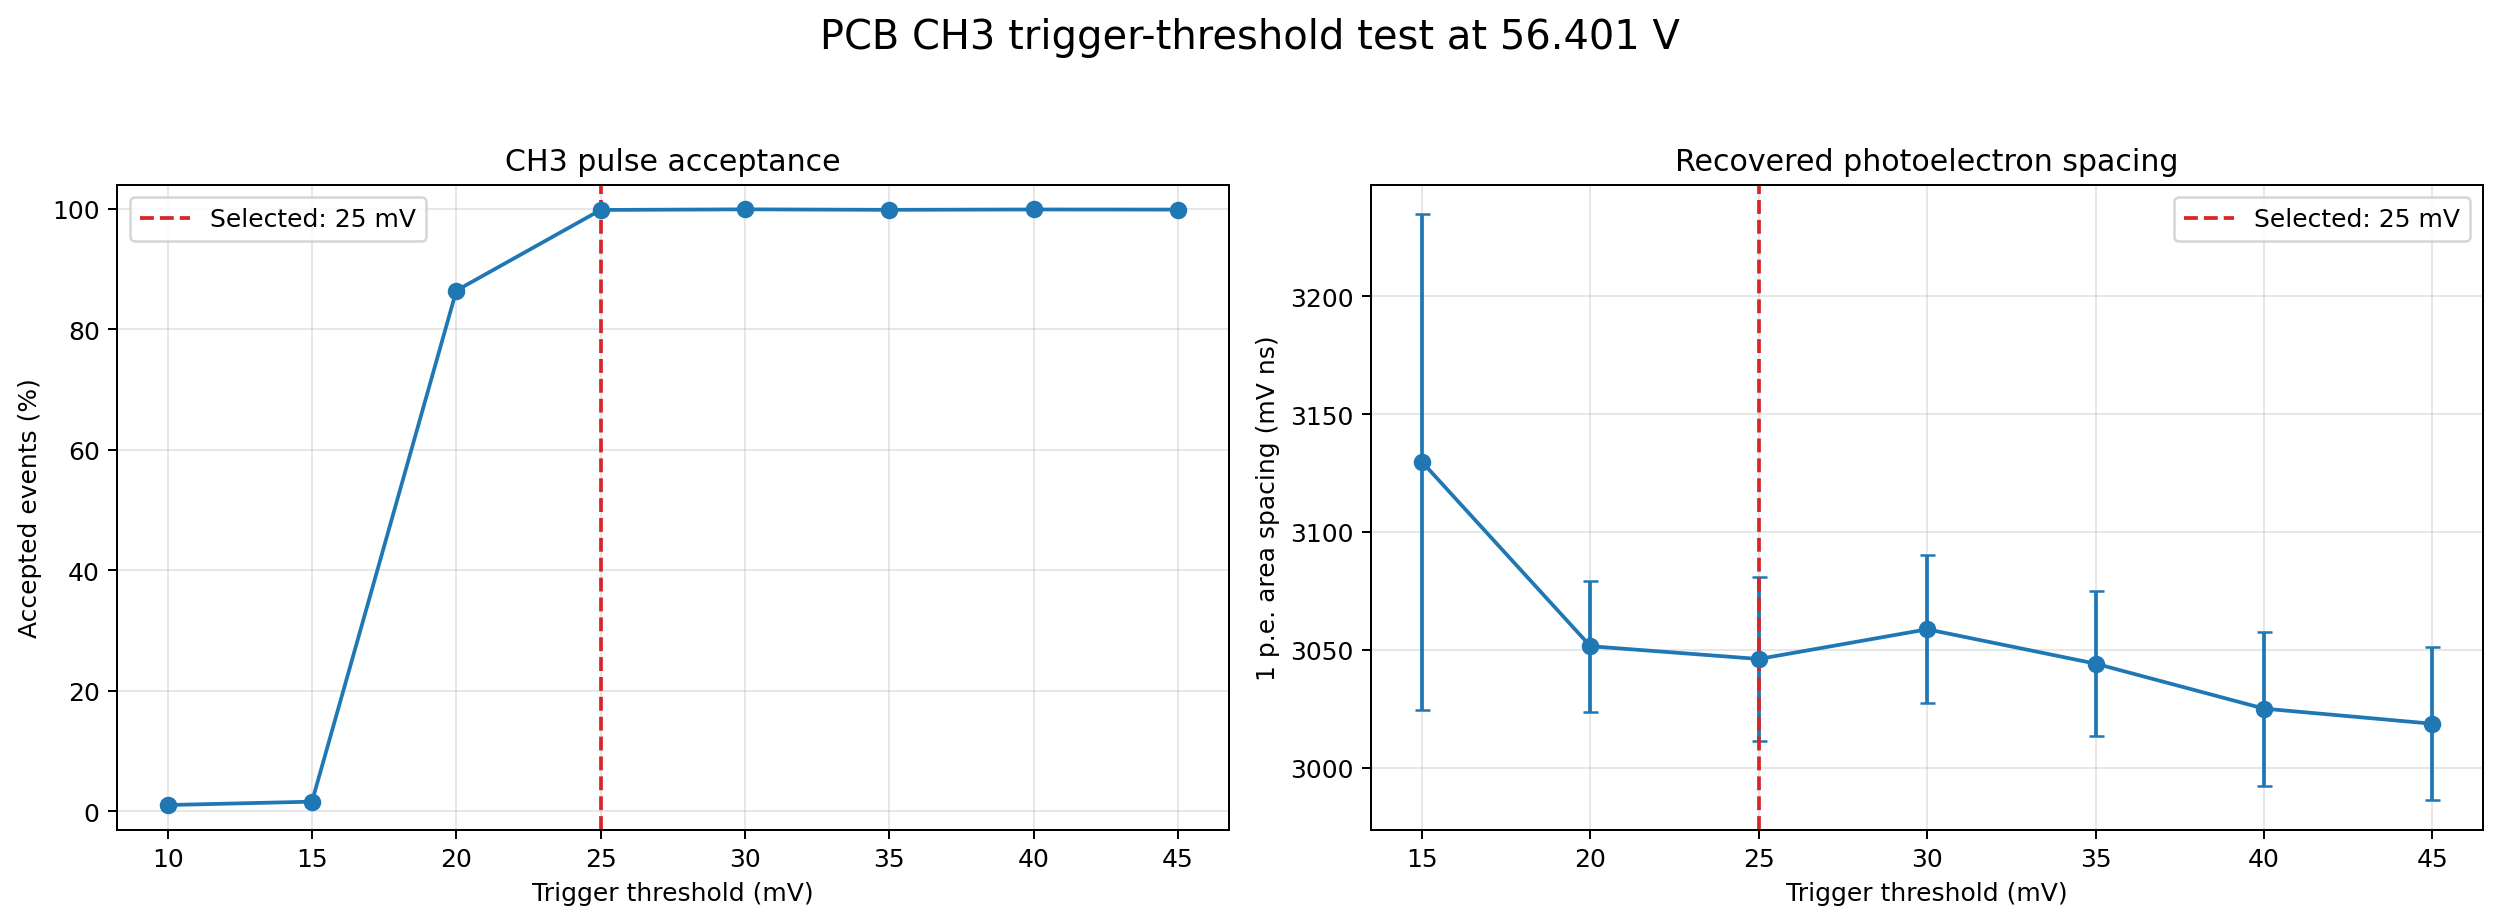
\includegraphics[width=0.92\linewidth]{ch3-trigger-selection.png}
  \caption{PCB CH3 acquisition acceptance and extracted spacing as the PicoScope trigger was varied. The stable high-acceptance region begins near \SI{25}{\milli\volt}.}
  \label{fig:ch3-trigger}
\end{figure}

\section{Waveform Processing}

\subsection{Event-by-event baseline}

Electronic offset was estimated for each event from pre-trigger samples. A robust procedure was used instead of a plain mean. The median and median absolute deviation were first calculated,

\begin{equation}
  \mathrm{MAD}=\operatorname{median}\left(\left|x_i-\operatorname{median}(x)\right|\right),
  \qquad
  \sigma_{\mathrm{robust}}=1.4826\,\mathrm{MAD}.
  \label{eq:mad}
\end{equation}

Outlying pre-trigger samples were removed and the baseline was recalculated. The corrected waveform was

\begin{equation}
  v(t)=V_{\mathrm{recorded}}(t)-V_{\mathrm{baseline}}.
\end{equation}

The robust estimate prevents one pickup transient or early pulse from moving the baseline of an entire event.

\subsection{Pulse location and integration}

The pulse maximum was searched for only within the expected prompt region. Searching the entire record can incorrectly select a late afterpulse or pickup transient. A three-point quadratic interpolation estimated the maximum between ADC samples. The integration gate in \cref{eq:pulse-area} then followed the measured peak time.

Waveforms were rejected when the baseline region was incomplete, the prompt maximum fell outside the permitted interval, the pulse failed the noise requirement, the integration gate left the recorded window, or the waveform touched the digitizer rail.

\subsection{Saturation and quality control}

Saturation was checked using waveform overlays and the relationship between height and area. Clipping is indicated when many traces share the same maximum, peak height stops increasing while area continues to change, or samples accumulate at the scope rail. A clipped spectrum cannot be repaired by recording more events; the range, gain, or bias must be changed.

The accepted-event fraction was also plotted against voltage. An abrupt acceptance change can indicate trigger selection rather than a real change in SiPM behavior.

\section{Photoelectron Spectrum Analysis}

\subsection{Historical peak-finding method}

The early analyses built a raw histogram and smoothed its bin counts with
\path{scipy.ndimage.gaussian_filter1d}. Candidate maxima were found with
\path{scipy.signal.find_peaks} and refined using a local Gaussian plus linear background fitted with
\path{scipy.optimize.curve_fit}. The refined centers were sorted, and combinations were tested for an approximately even sequence.

For histogram counts $H(x_i)$, Gaussian smoothing has the form

\begin{equation}
  S(x)=\frac{\sum_i H(x_i)\exp\left[-(x-x_i)^2/(2\sigma_s^2)\right]}
  {\sum_i \exp\left[-(x-x_i)^2/(2\sigma_s^2)\right]}.
\end{equation}

The smoothed curve was used only to locate candidates. Peak centers were refined against the unsmoothed bins. This distinction matters because smoothing does not add information to the data.

\subsection{Pedestal-constrained comb model}

The current primary method fits several p.e. populations together. Their centers share one spacing,

\begin{equation}
  \mu_n=\mu_0+n\Delta Q.
  \label{eq:comb-centers}
\end{equation}

The pedestal location and width are constrained by the independent pedestal acquisition. Population amplitudes and widths can vary. The optimization uses \texttt{scipy.optimize.least\_squares} with a Poisson-deviance residual for histogram counts. Several starting spacings are tried to test stability.

The multi-population model is compared with a single broad population using the Bayesian information criterion,

\begin{equation}
  \mathrm{BIC}=D+k\ln N,
\end{equation}

where $D$ is the deviance, $k$ the number of model parameters, and $N$ the number of fitted observations used by the implementation. In the lower-bias study, a comb point required $\Delta\mathrm{BIC}\geq10$ together with stable spacing and separated neighboring populations.

\subsection{Why every visible maximum is not a p.e. peak}

A p.e. sequence should be approximately periodic. A small first population followed by a larger second population can be physically reasonable because the trigger can suppress small pulses and optical crosstalk can move events into higher populations. However, two nearby maxima inside one expected population can also result from pulse-shape variation, pickup, or over-flexible peak finding. The analysis therefore uses the complete spacing pattern and fit stability rather than accepting every local maximum.

\begin{figure}[htbp]
  \centering
  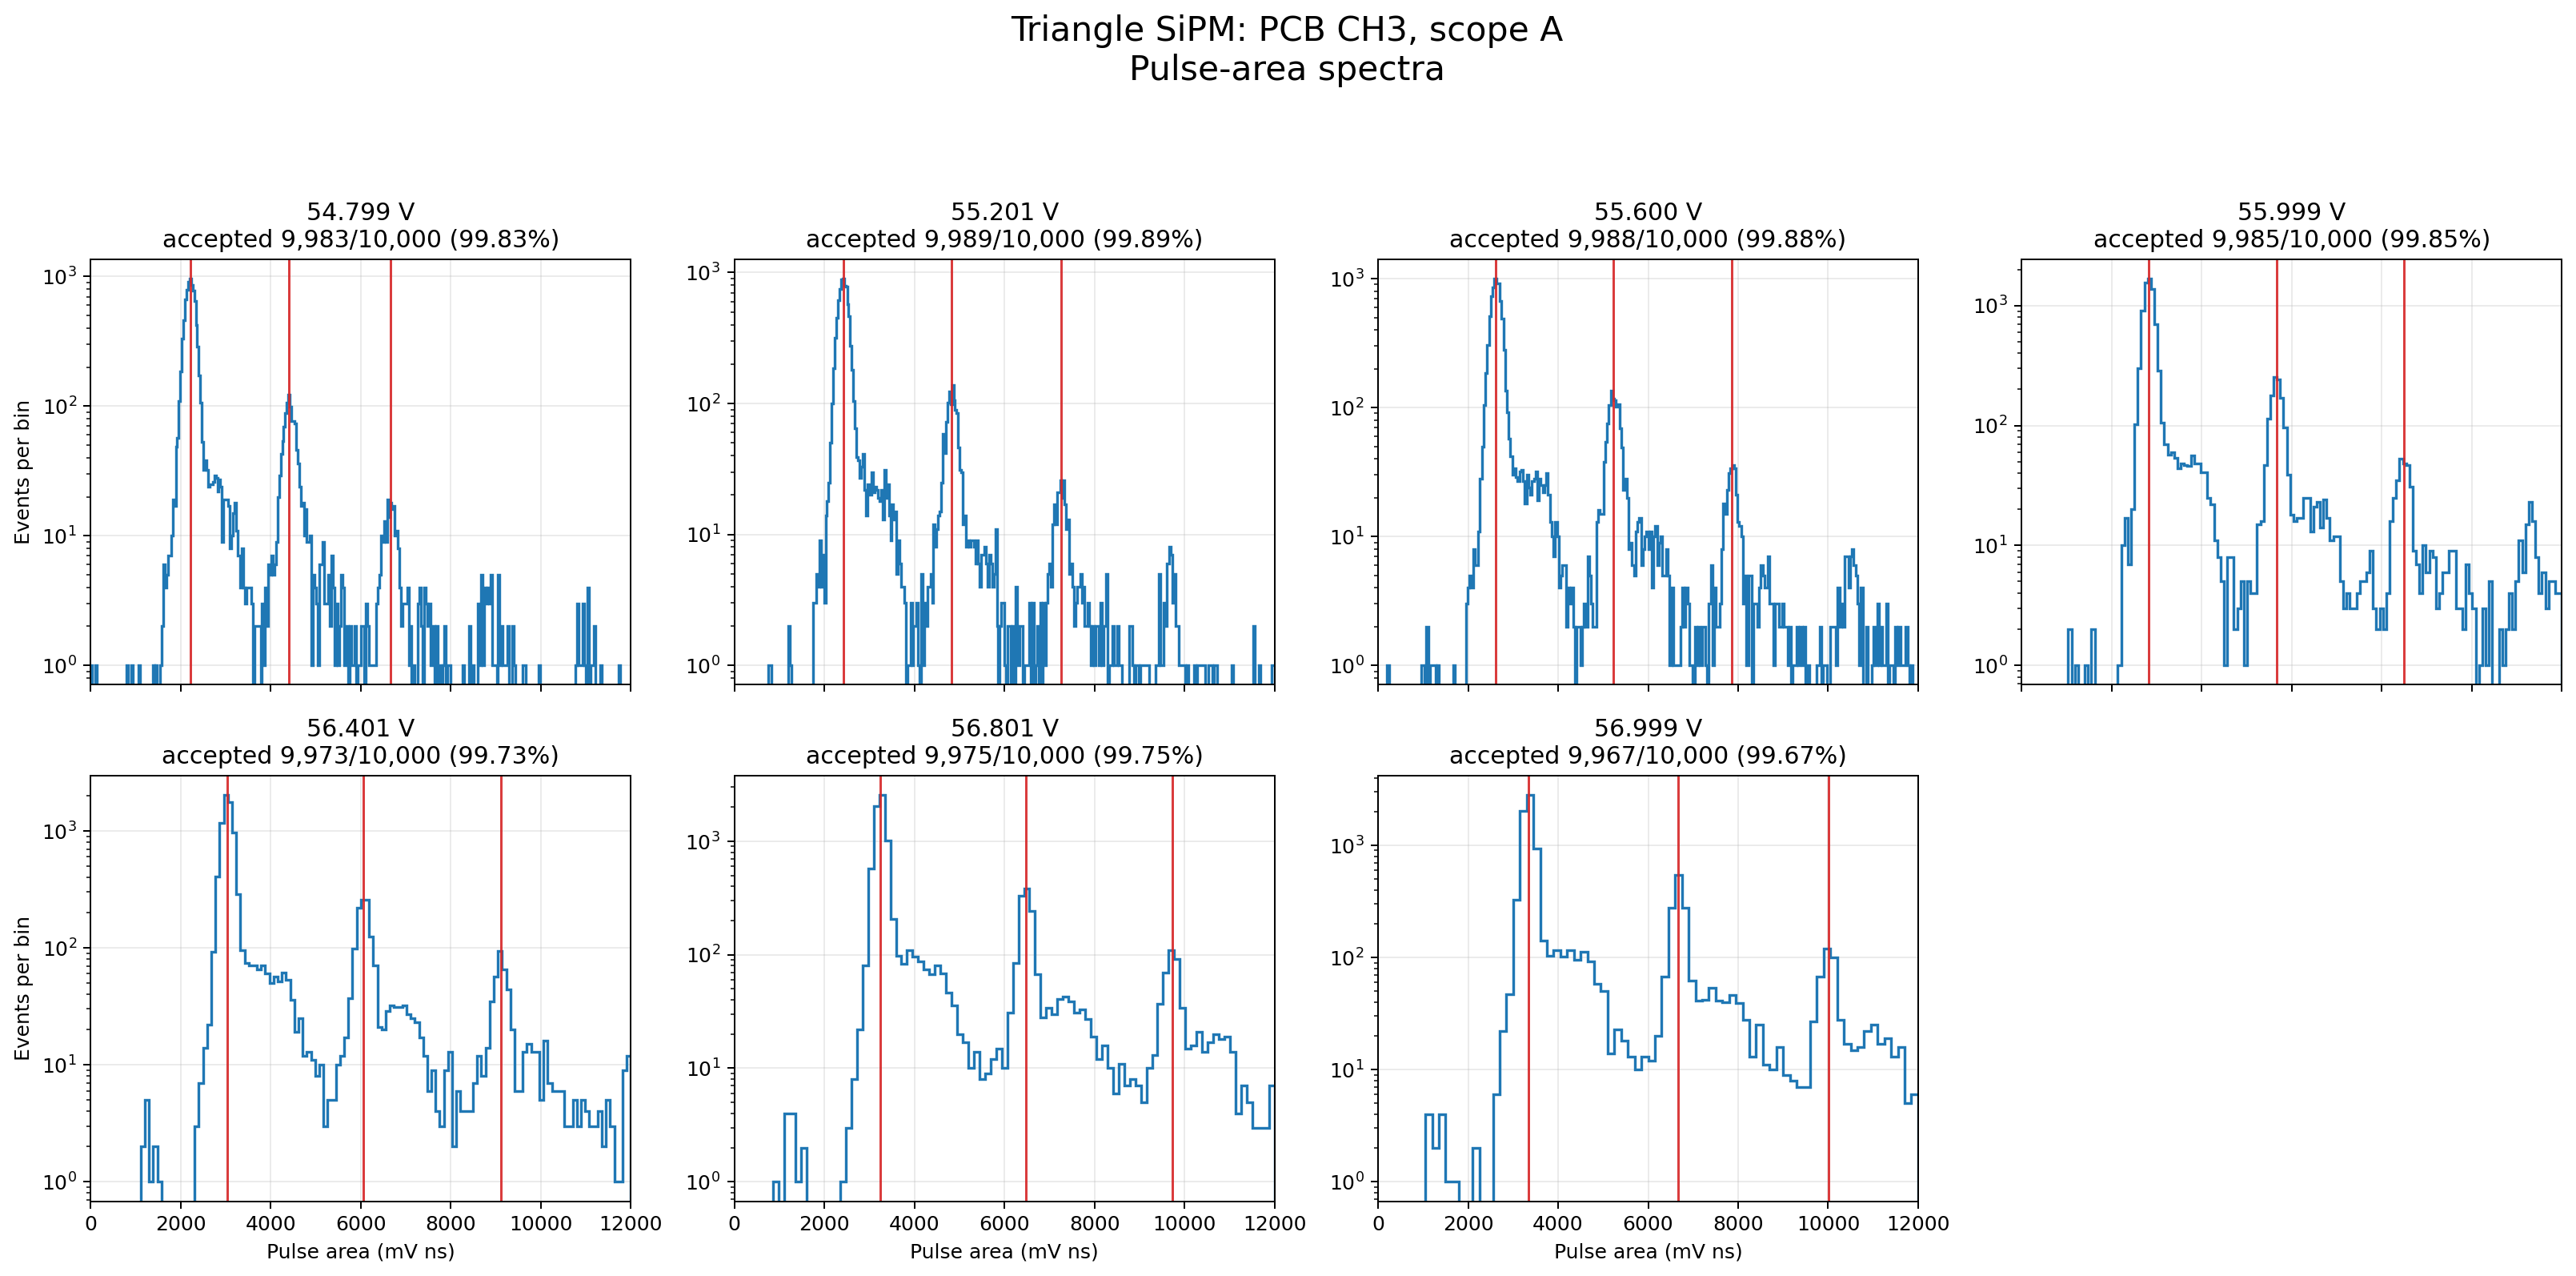
\includegraphics[width=0.98\linewidth]{triangle-spectra.png}
  \caption{Pulse-area spectra from the Triangle SiPM across the clean bias scan. Raw histogram structure and the fitted population sequence were inspected at each voltage.}
  \label{fig:triangle-spectra}
\end{figure}

\begin{figure}[htbp]
  \centering
  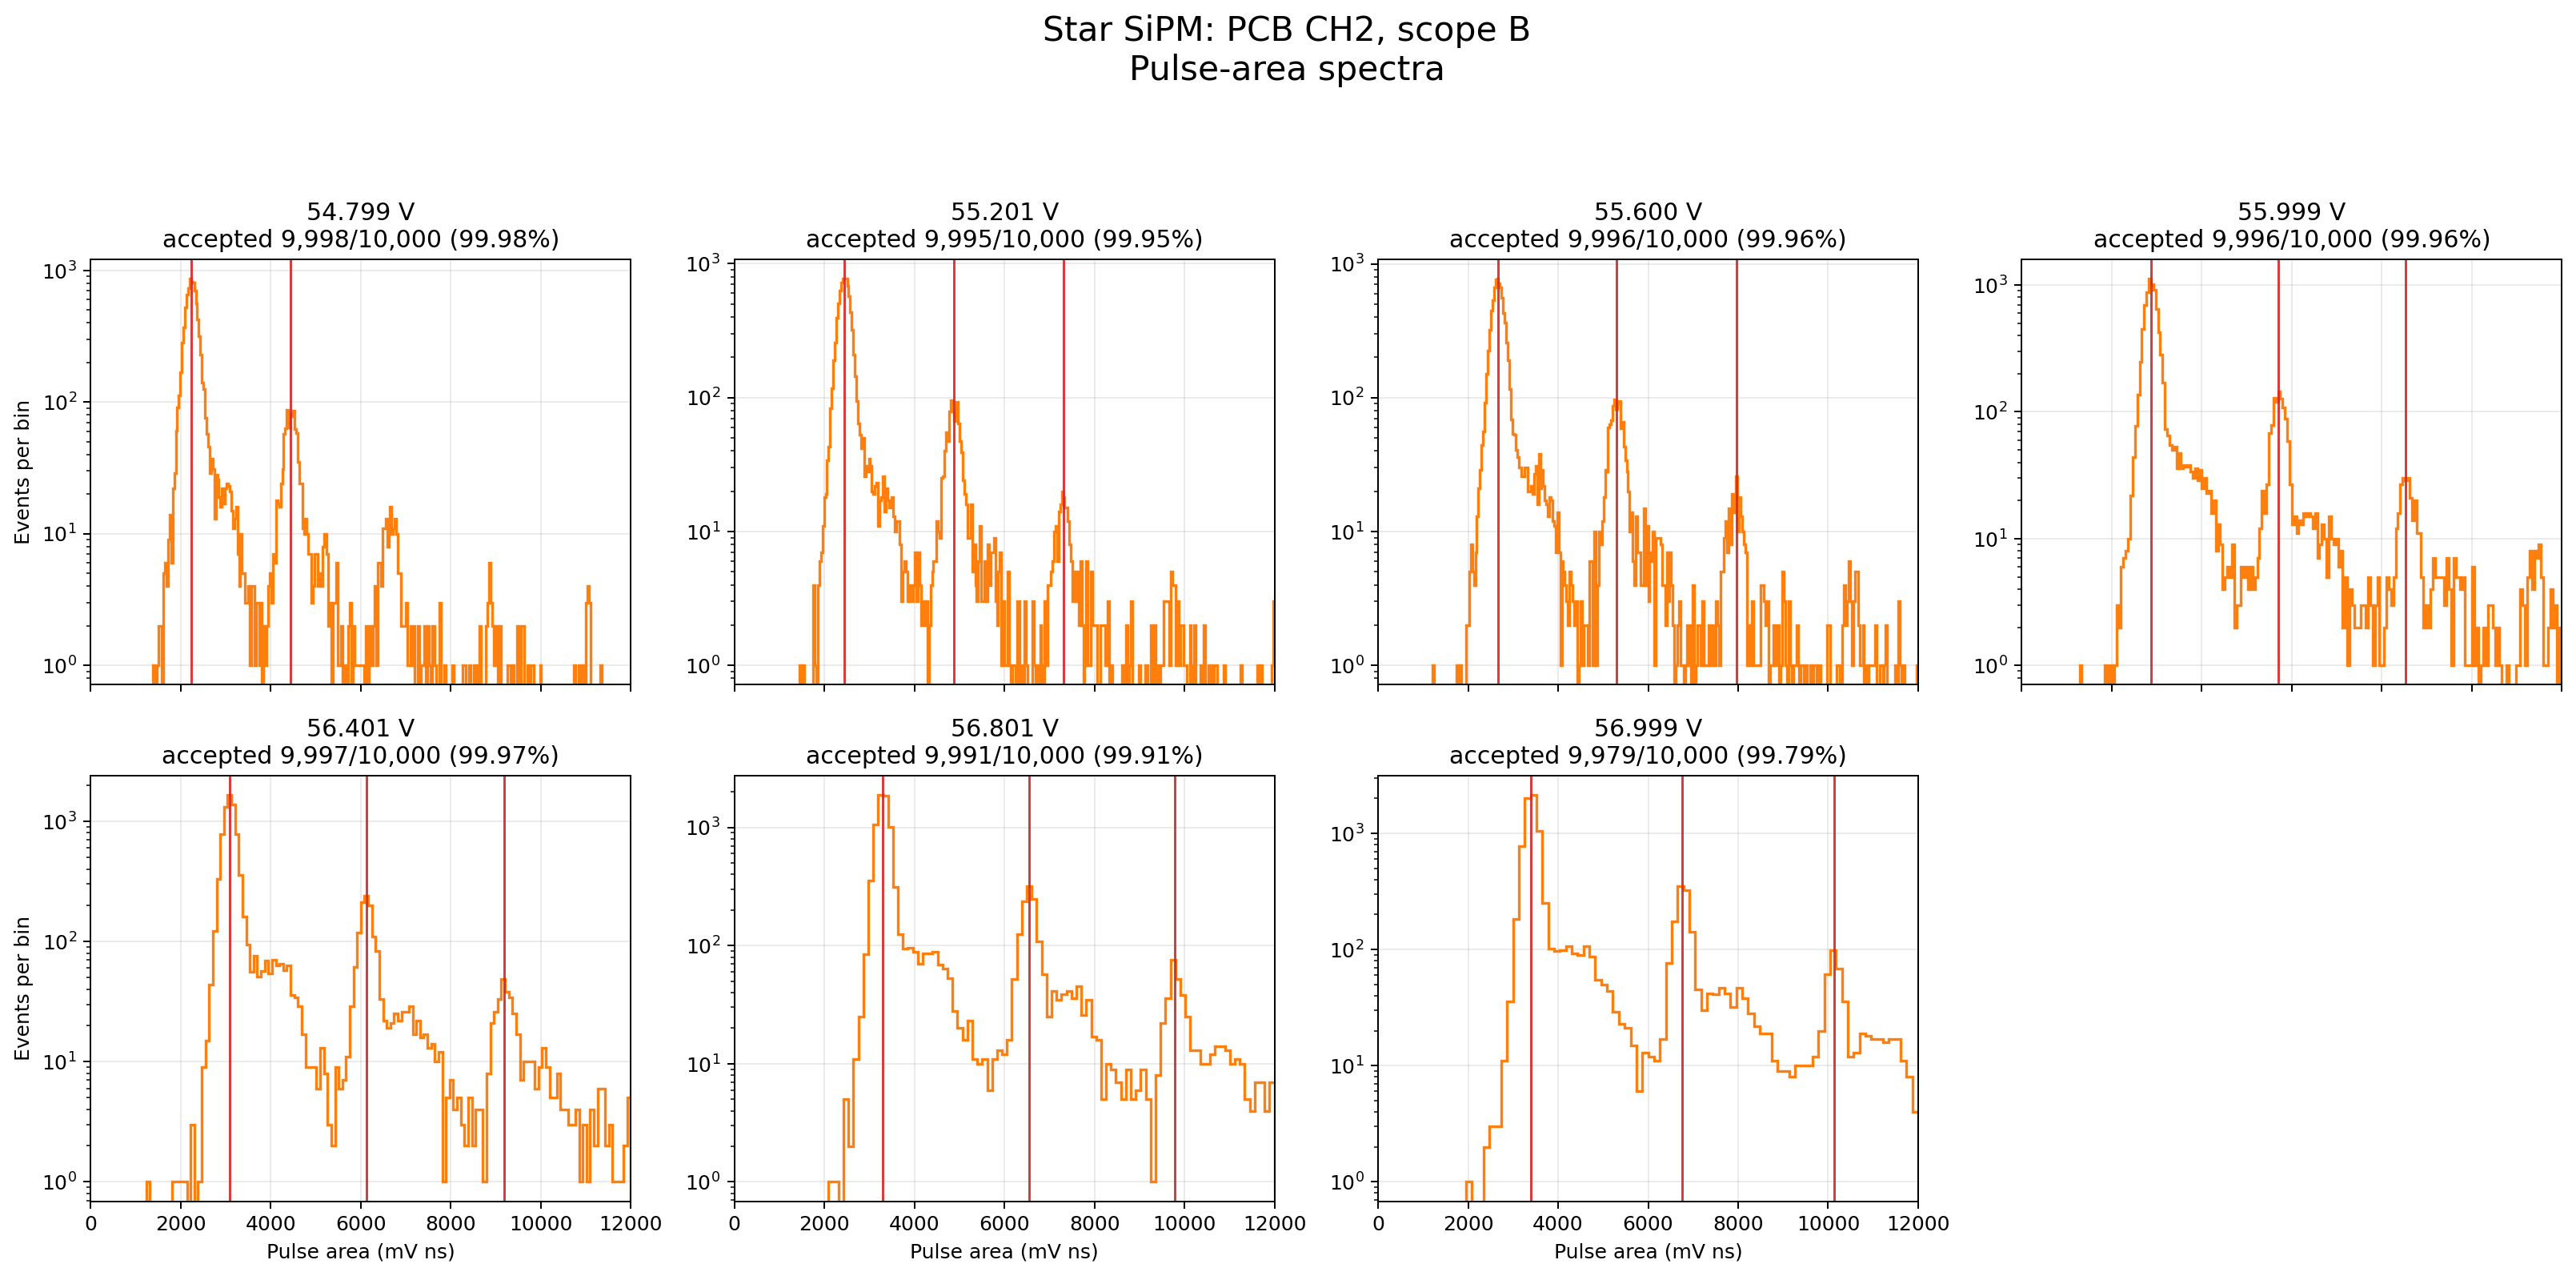
\includegraphics[width=0.98\linewidth]{star-spectra.png}
  \caption{Pulse-area spectra from the Star SiPM across the clean bias scan.}
  \label{fig:star-spectra}
\end{figure}

\subsection{Spacing and breakdown-voltage uncertainties}

The comb-fit covariance gives the statistical uncertainty of $\Delta Q$ under the selected model. The spacing points are then fitted against bias with an uncertainty floor so that one unrealistically precise point cannot dominate. If the point scatter exceeds the stated errors, an additional vertical scatter term is included.

The covariance of slope and intercept is propagated through $\vbr=-b/m$. The fit is also repeated while removing one voltage at a time. A large movement under this leave-one-out test indicates that the nominal regression uncertainty is not a reliable description of the measurement.

\section{Breakdown-Voltage Results}

\subsection{Original SiPM pair}

The original SIPM1 and SIPM2 were measured in three independent scans. Each main scan used six bias points from approximately 53.4 to \SI{56.9}{\volt} and 10,000 waveforms per SiPM per point. The combined internal results at \SI{20}{\degreeCelsius} were:

\begin{table}[htbp]
  \centering
  \caption{Breakdown-voltage results for the original SiPM pair.}
  \label{tab:original-results}
  \begin{tabular}{lccc}
    \toprule
    Device & $\vbr$ (V) & Area-spacing slope (mV ns/V) & $R^2$ \\
    \midrule
    SIPM1 & $50.637\pm0.037$ & 532.5 & 0.9997 \\
    SIPM2 & $51.988\pm0.103$ & 555.9 & 0.9976 \\
    \bottomrule
  \end{tabular}
\end{table}

The two devices have clearly different operational intercepts on the present bias scale. Applying one common voltage would therefore place them at different nominal overvoltages.

An interleaved scan tested new voltage points against previously frozen lines. The new intercepts, \SI{50.6466(374)}{\volt} and \SI{52.0662(633)}{\volt}, were compatible with the frozen values. This gave an important check that the fitted lines were not only reproducing the exact voltage points used to create them.

\begin{figure}[htbp]
  \centering
  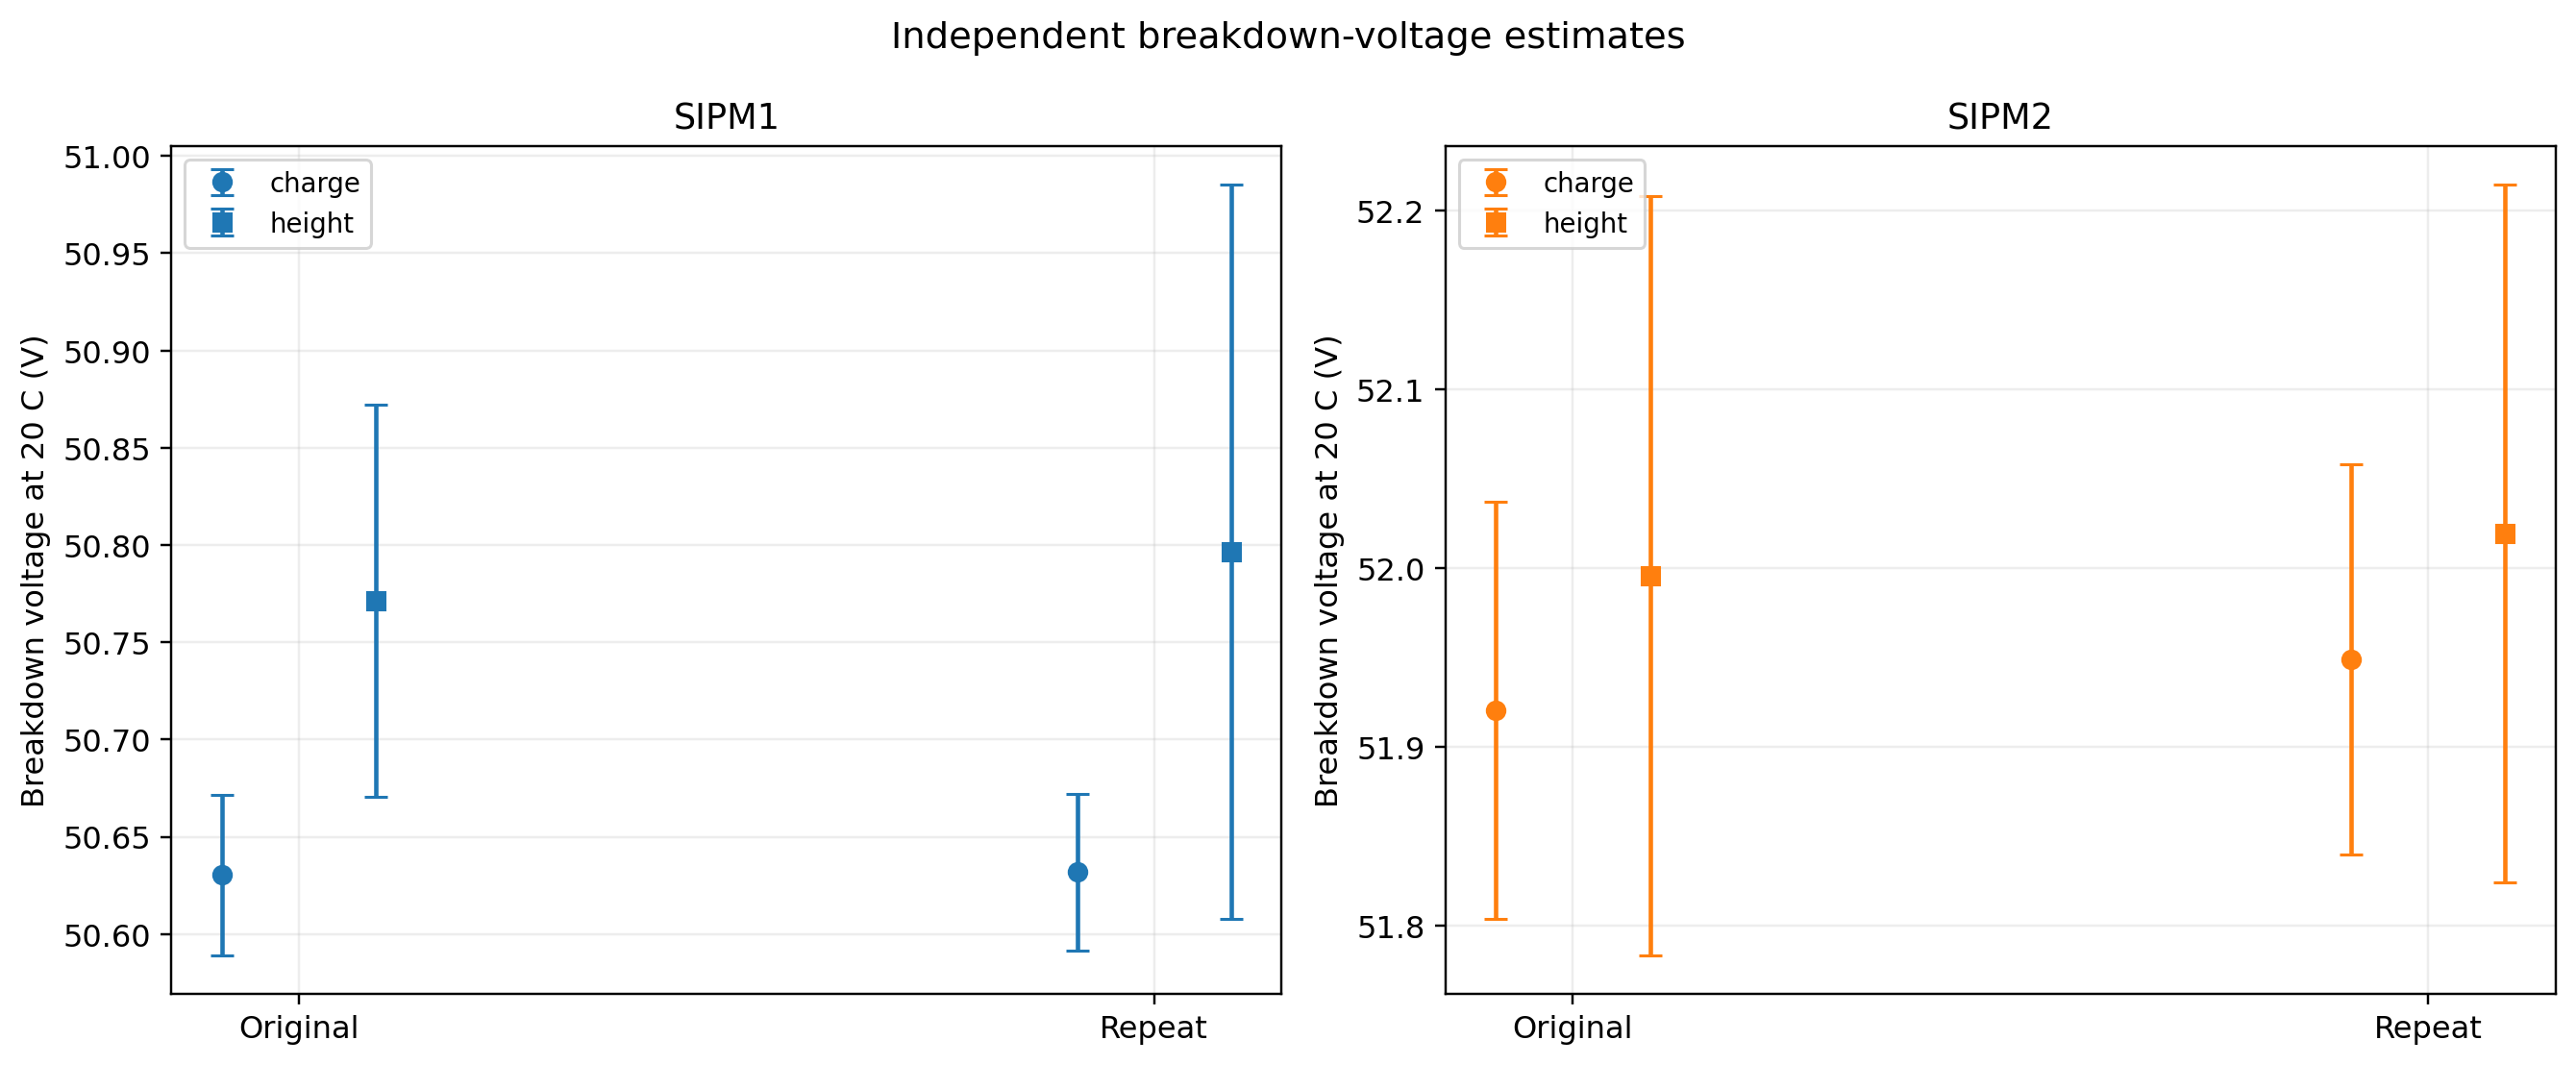
\includegraphics[width=0.94\linewidth]{original-repeatability.png}
  \caption{Breakdown-voltage repeatability for the original SiPM pair.}
  \label{fig:original-repeatability}
\end{figure}

\subsection{Lower-bias limit}

A separate scan covered 52.0 to \SI{53.4}{\volt} in \SI{0.2}{\volt} steps. The continuous stable region began at \SI{52.6}{\volt} for SIPM1 and \SI{53.2}{\volt} for SIPM2. Below those values, neighboring populations overlapped, trigger acceptance decreased, or the fitted spacing depended strongly on starting values.

For SIPM1, adding every apparently resolved low-bias point moved the fitted intercept from 50.630 to \SI{50.800}{\volt} and increased the required intrinsic charge scatter from 7.9 to \SI{25.5}{\milli\volt\nano\second}. The added points therefore introduced low-end selection bias rather than useful leverage.

\begin{figure}[htbp]
  \centering
  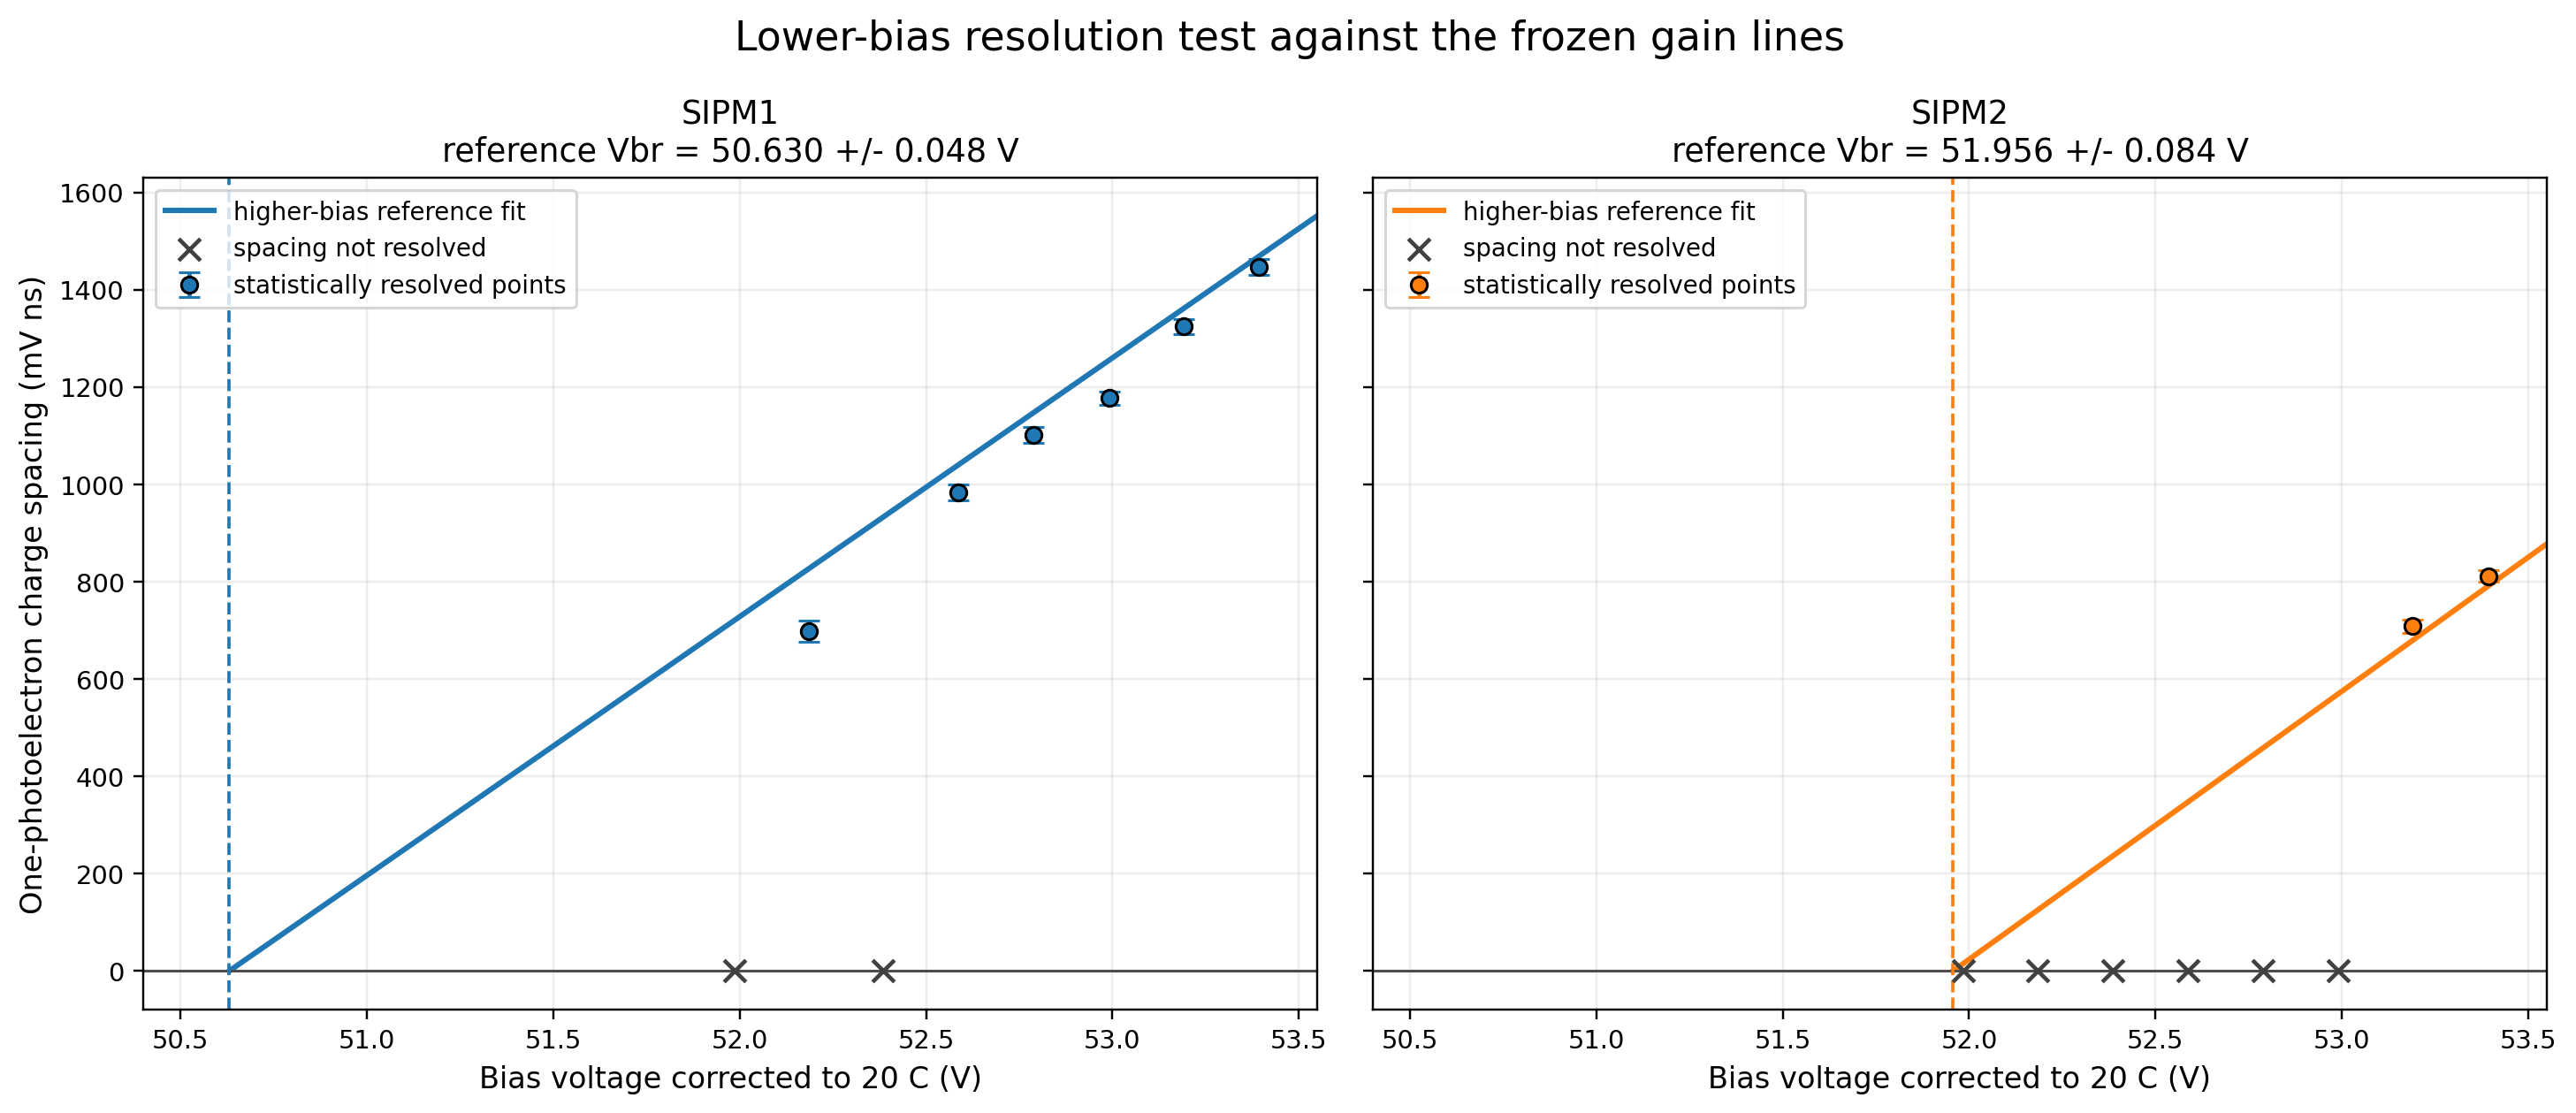
\includegraphics[width=0.96\linewidth]{lower-bias-resolution.png}
  \caption{Lower-bias resolution tests. Points close to breakdown were retained only when the multi-population structure remained statistically supported and stable.}
  \label{fig:lower-bias}
\end{figure}

\subsection{Triangle and Star pair}

After the CH3 trigger study, both physical SiPMs were measured over seven matched bias points with 10,000 waveforms at each point. The complete scan was then repeated independently. The temperature during the repeat ranged from 20.365 to \SI{20.462}{\degreeCelsius}.

\begin{table}[htbp]
  \centering
  \caption{Two clean measurements of the Triangle and Star SiPMs. Uncertainties are internal waveform-analysis uncertainties.}
  \label{tab:triangle-star-runs}
  \begin{tabular}{lccc}
    \toprule
    Device & First scan $\vbr$ (V) & Repeat $\vbr$ (V) & Weighted $\vbr$ (V) \\
    \midrule
    SiPM 1 (Triangle) & $50.534\pm0.113$ & $50.486\pm0.121$ & $50.512\pm0.083$ \\
    SiPM 2 (Star) & $50.667\pm0.097$ & $50.488\pm0.092$ & $50.574\pm0.067$ \\
    \bottomrule
  \end{tabular}
\end{table}

The repeat scan accepted 69,860 of 70,000 Triangle waveforms and 69,952 of 70,000 Star waveforms. The repeat area-spacing slopes were $513.32\pm12.44$ and $515.68\pm9.40$ \si{\milli\volt\nano\second\per\volt}, respectively. The mean absolute point-by-point changes in spacing were 0.66\% and 0.59\%.

The Star-minus-Triangle breakdown-voltage difference is

\begin{equation}
  \Delta\vbr = \SI{0.062(106)}{\volt},
\end{equation}

which is a $0.58\sigma$ difference. The current data therefore do not show a statistically significant difference between these two devices.

\begin{figure}[htbp]
  \centering
  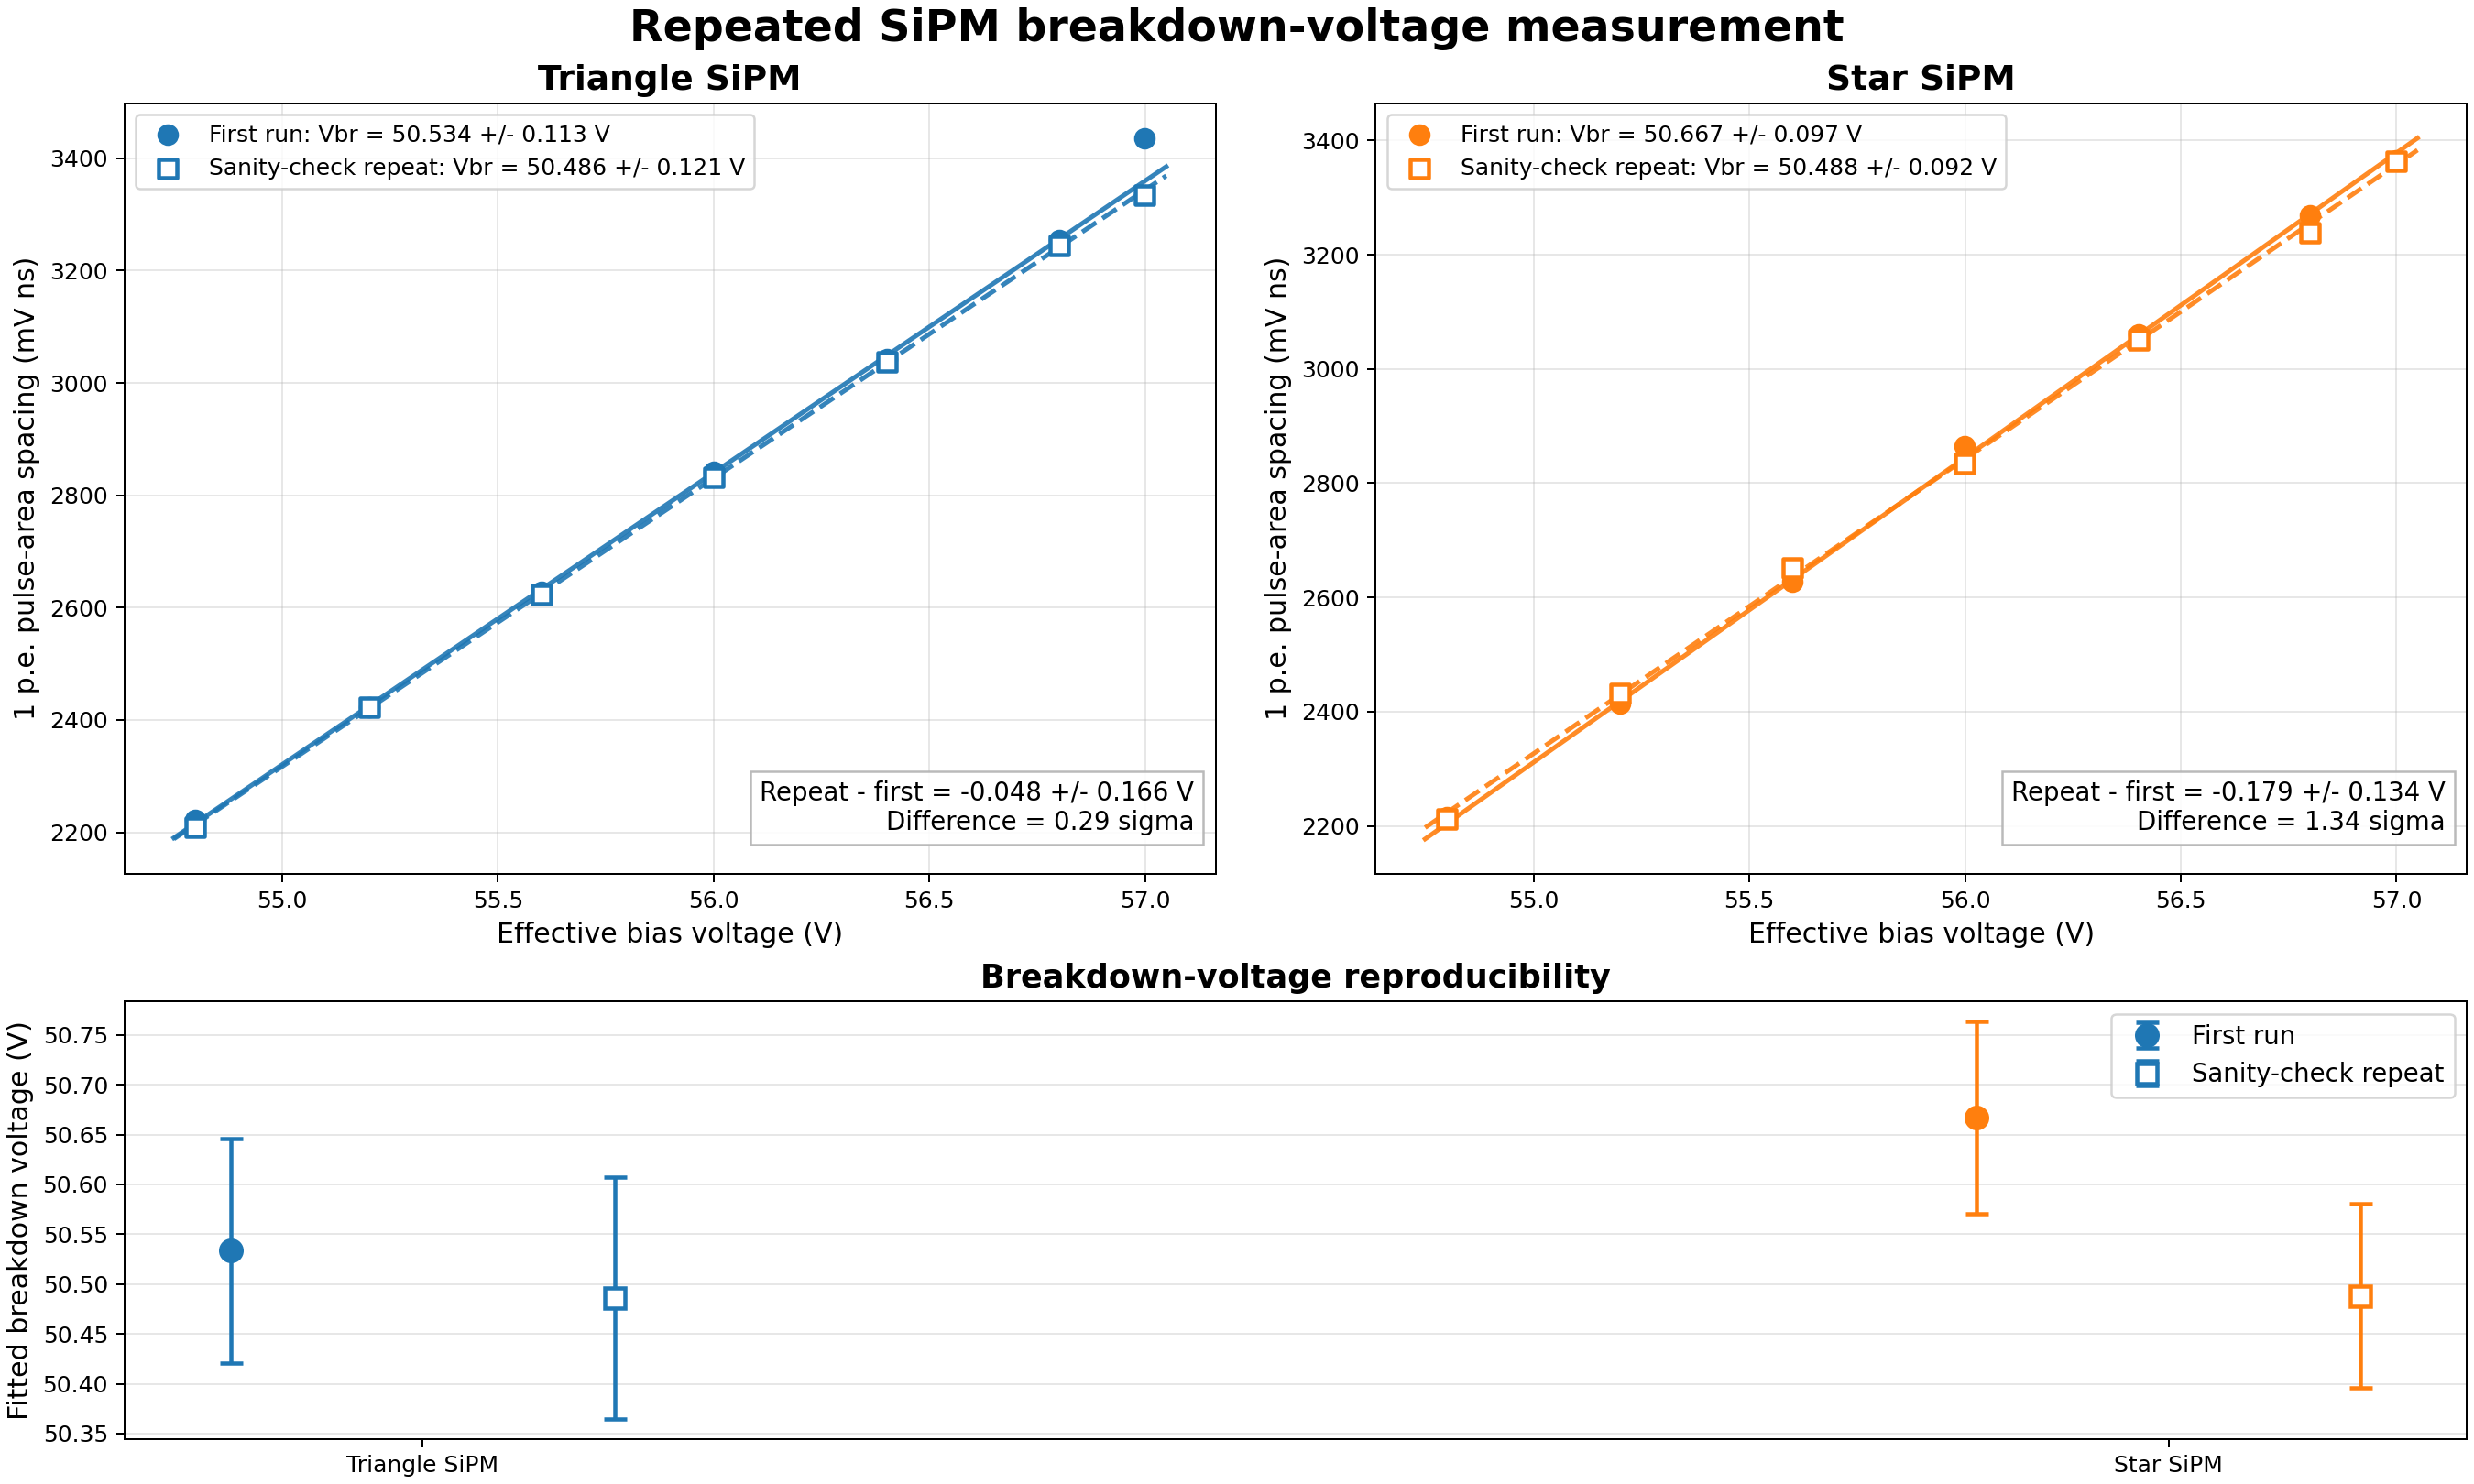
\includegraphics[width=0.98\linewidth]{triangle-star-repeatability.png}
  \caption{First and repeated breakdown-voltage measurements for the Triangle and Star SiPMs. The channel-switched and repeated points provide a test of physical-device identity and run-to-run stability.}
  \label{fig:triangle-star-repeatability}
\end{figure}

\subsection{Provisional operating points}

A controlled starting point is \SI{3.0}{\volt} above the measured breakdown voltage. Near \SI{20.4}{\degreeCelsius}, this gives approximately

\begin{table}[htbp]
  \centering
  \caption{Provisional operating points for the Triangle and Star SiPMs.}
  \label{tab:operating-points}
  \begin{tabular}{lcc}
    \toprule
    Device & Weighted $\vbr$ (V) & Provisional $\vbr+\SI{3.0}{\volt}$ setting (V) \\
    \midrule
    SiPM 1 (Triangle) & $50.512\pm0.083$ & 53.51 \\
    SiPM 2 (Star) & $50.574\pm0.067$ & 53.57 \\
    \bottomrule
  \end{tabular}
\end{table}

These are working settings on the present bias calibration. They should not be interpreted as traceable terminal voltages until the high side and channel low sides are measured directly with a calibrated high-impedance instrument.

\section{EPIC-Triggered Zero-Event Study}

\subsection{Purpose}

The breakdown-voltage measurement equalizes nominal overvoltage. It does not test the final response to scintillation light. Two SiPMs at the same overvoltage can still differ in photon-detection efficiency, dark-count rate, correlated noise, fibre coupling, or amplifier response.

The zero-event study uses two EPIC tiles as reference counters. A top and bottom EPIC coincidence selects a particle crossing the central region. The two GSU gLOWCOST tile waveforms are then examined for a pulse in the expected time window.

\begin{figure}[htbp]
  \centering
  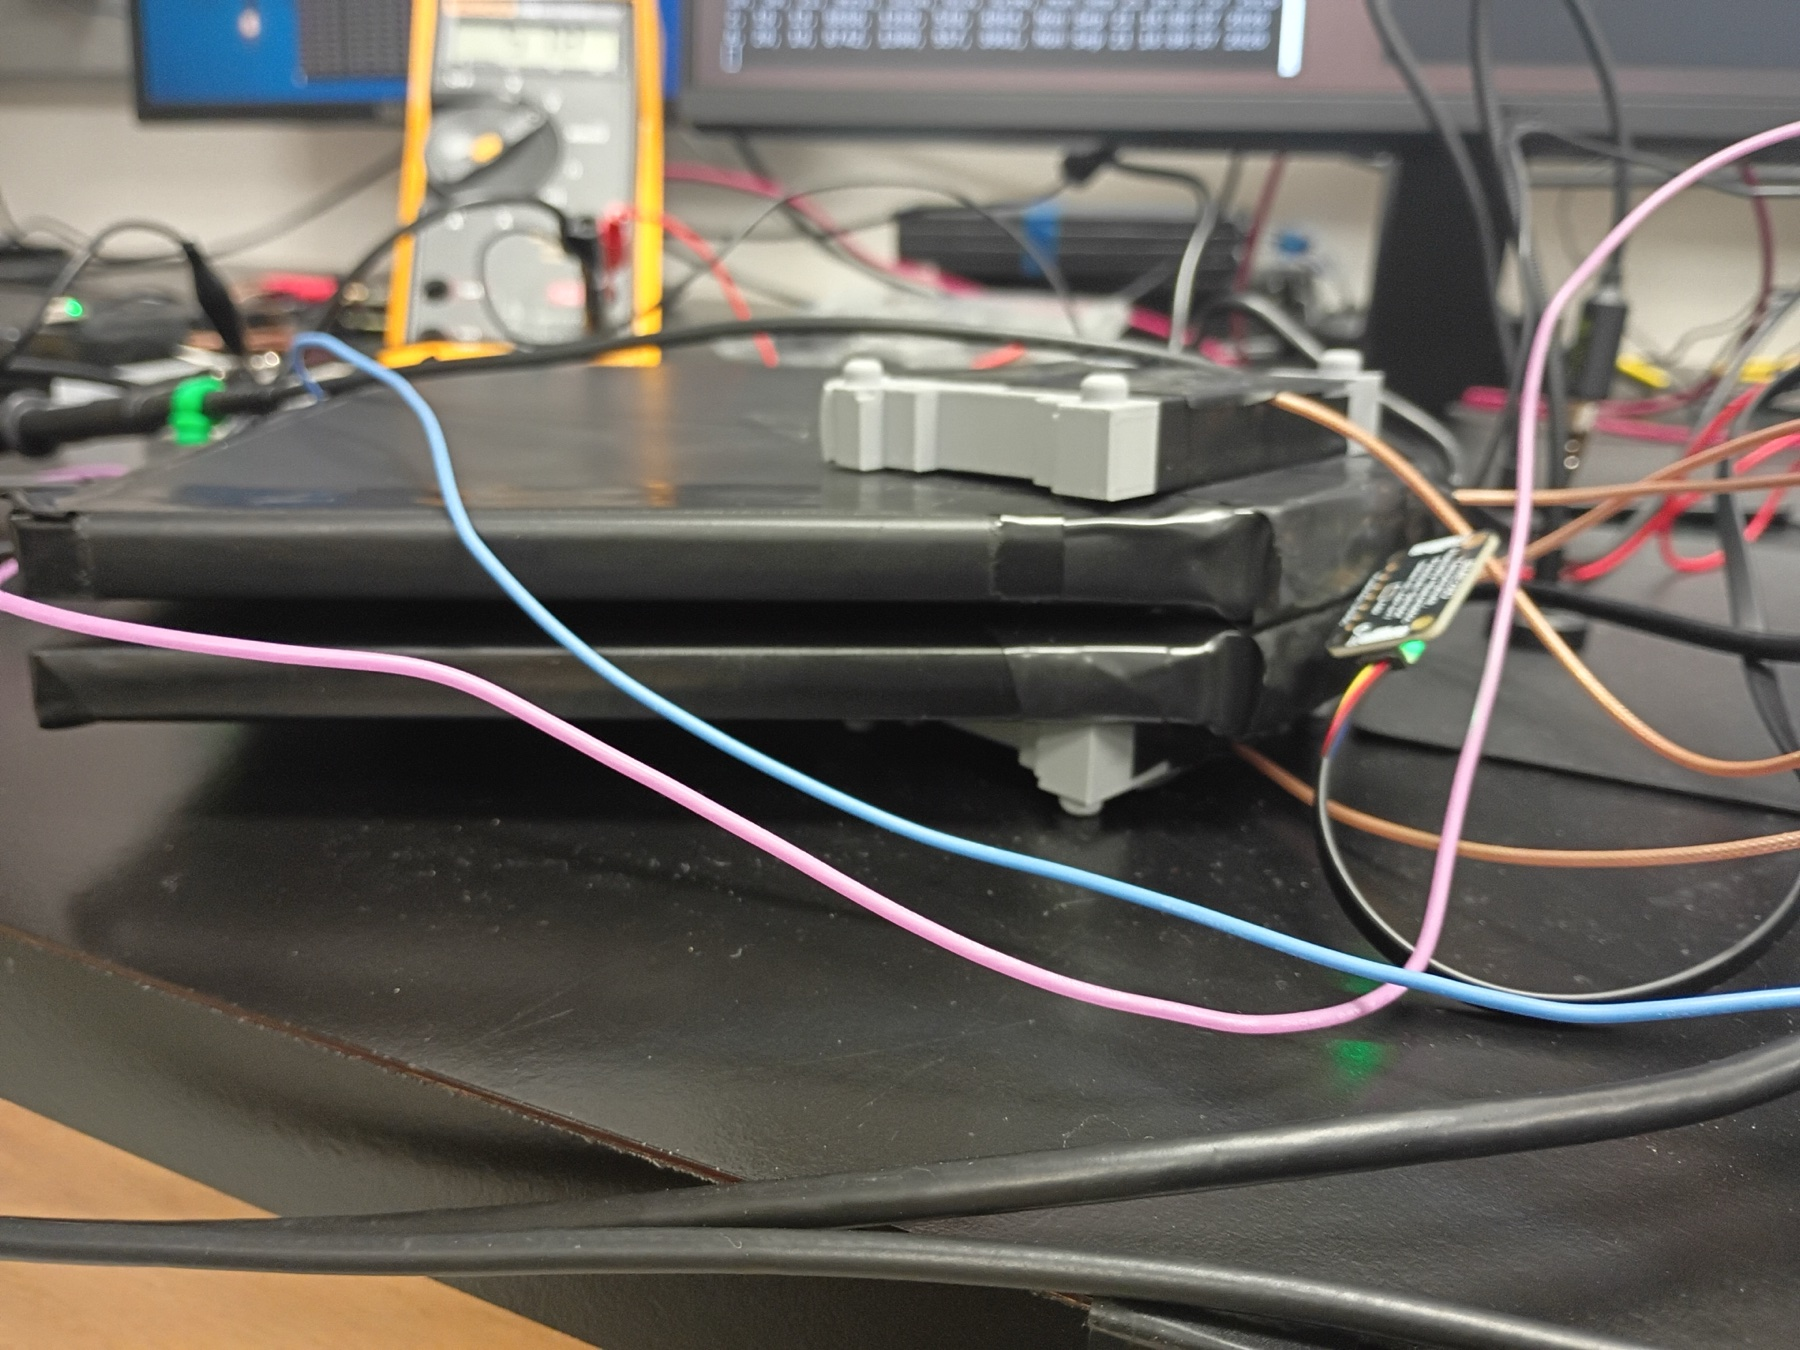
\includegraphics[width=0.88\linewidth]{scintillator-stack.jpg}
  \caption{Two GSU gLOWCOST tiles placed between the top and bottom EPIC reference tiles.}
  \label{fig:scintillator-stack}
\end{figure}

The current physical mapping is shown in \cref{tab:zero-event-map}.

\begin{table}[htbp]
  \centering
  \caption{Channel mapping for the EPIC-triggered GSU gLOWCOST measurement.}
  \label{tab:zero-event-map}
  \begin{tabular}{llll}
    \toprule
    Position & SiPM label & PCB channel & Scope channel \\
    \midrule
    Top EPIC tile & not individually calibrated & CH0 & C \\
    Top GSU gLOWCOST tile & SiPM 1 (Triangle) & CH2 & A \\
    Bottom GSU gLOWCOST tile & SiPM 2 (Star) & CH3 & B \\
    Bottom EPIC tile & not individually calibrated & CH1 & D \\
    \bottomrule
  \end{tabular}
\end{table}

\subsection{Zero fraction and dark correction}

For each EPIC coincidence, the GSU gLOWCOST signal gate is classified as zero or nonzero using a boundary between the pedestal and one-p.e. response. An equal-duration dark-time window from the same waveform estimates accidental dark pulses and electronic-noise crossings.

Let $f_s$ be the measured zero fraction in the expected signal gate and $f_d$ the zero fraction in the dark-time gate. If the scintillation response and accidental dark activity are independent, an empty signal gate requires both no detected scintillation response and no accidental pulse. Therefore,

\begin{equation}
  P_0(\text{scintillation})=\frac{f_s}{f_d},
  \qquad
  \epsilon_{\mathrm{chain}}=1-\frac{f_s}{f_d}.
  \label{eq:zero-efficiency}
\end{equation}

The correction prevents an accidental dark pulse from being counted as successful scintillation detection.

If detected primary photoelectrons follow a Poisson distribution with mean $\mu$, then

\begin{equation}
  P(0)=e^{-\mu},
  \qquad
  \mu=-\ln P(0).
  \label{eq:zero-poisson}
\end{equation}

For cosmic-ray scintillation, $\mu$ should be described as a zero-equivalent occupancy rather than an absolute photon yield. Muons do not all deposit identical energy or follow identical paths, and the optical collection varies with position. A pulsed LED with controlled light is required for a cleaner relative PDE measurement.

\subsection{Pilot observations}

The first EPIC coincidence attempt used high analogue thresholds and produced only auto-trigger records, showing that the condition was too strict. Later single-channel tests showed that scope D pulses were smaller than scope C pulses. An HV-off control removed the live pulse population, confirming that the observed coincident signals were detector generated rather than a persistent scope artifact.

A 5,000-event development run used the following provisional reference cuts:

\begin{itemize}[leftmargin=*]
  \item scope C positive excursion of at least \SI{3000}{\milli\volt};
  \item scope D positive excursion of at least \SI{120}{\milli\volt}; and
  \item absolute C--D peak-time difference no greater than \SI{40}{\nano\second}.
\end{itemize}

Six events passed these strict cuts in \SI{81.49}{\second}, corresponding to approximately 4.4 events per minute. Four of the six showed excursions above \SI{200}{\milli\volt} in both GSU gLOWCOST channels. This sample demonstrated the geometry and timing logic but was too small for an efficiency result.

\begin{figure}[htbp]
  \centering
  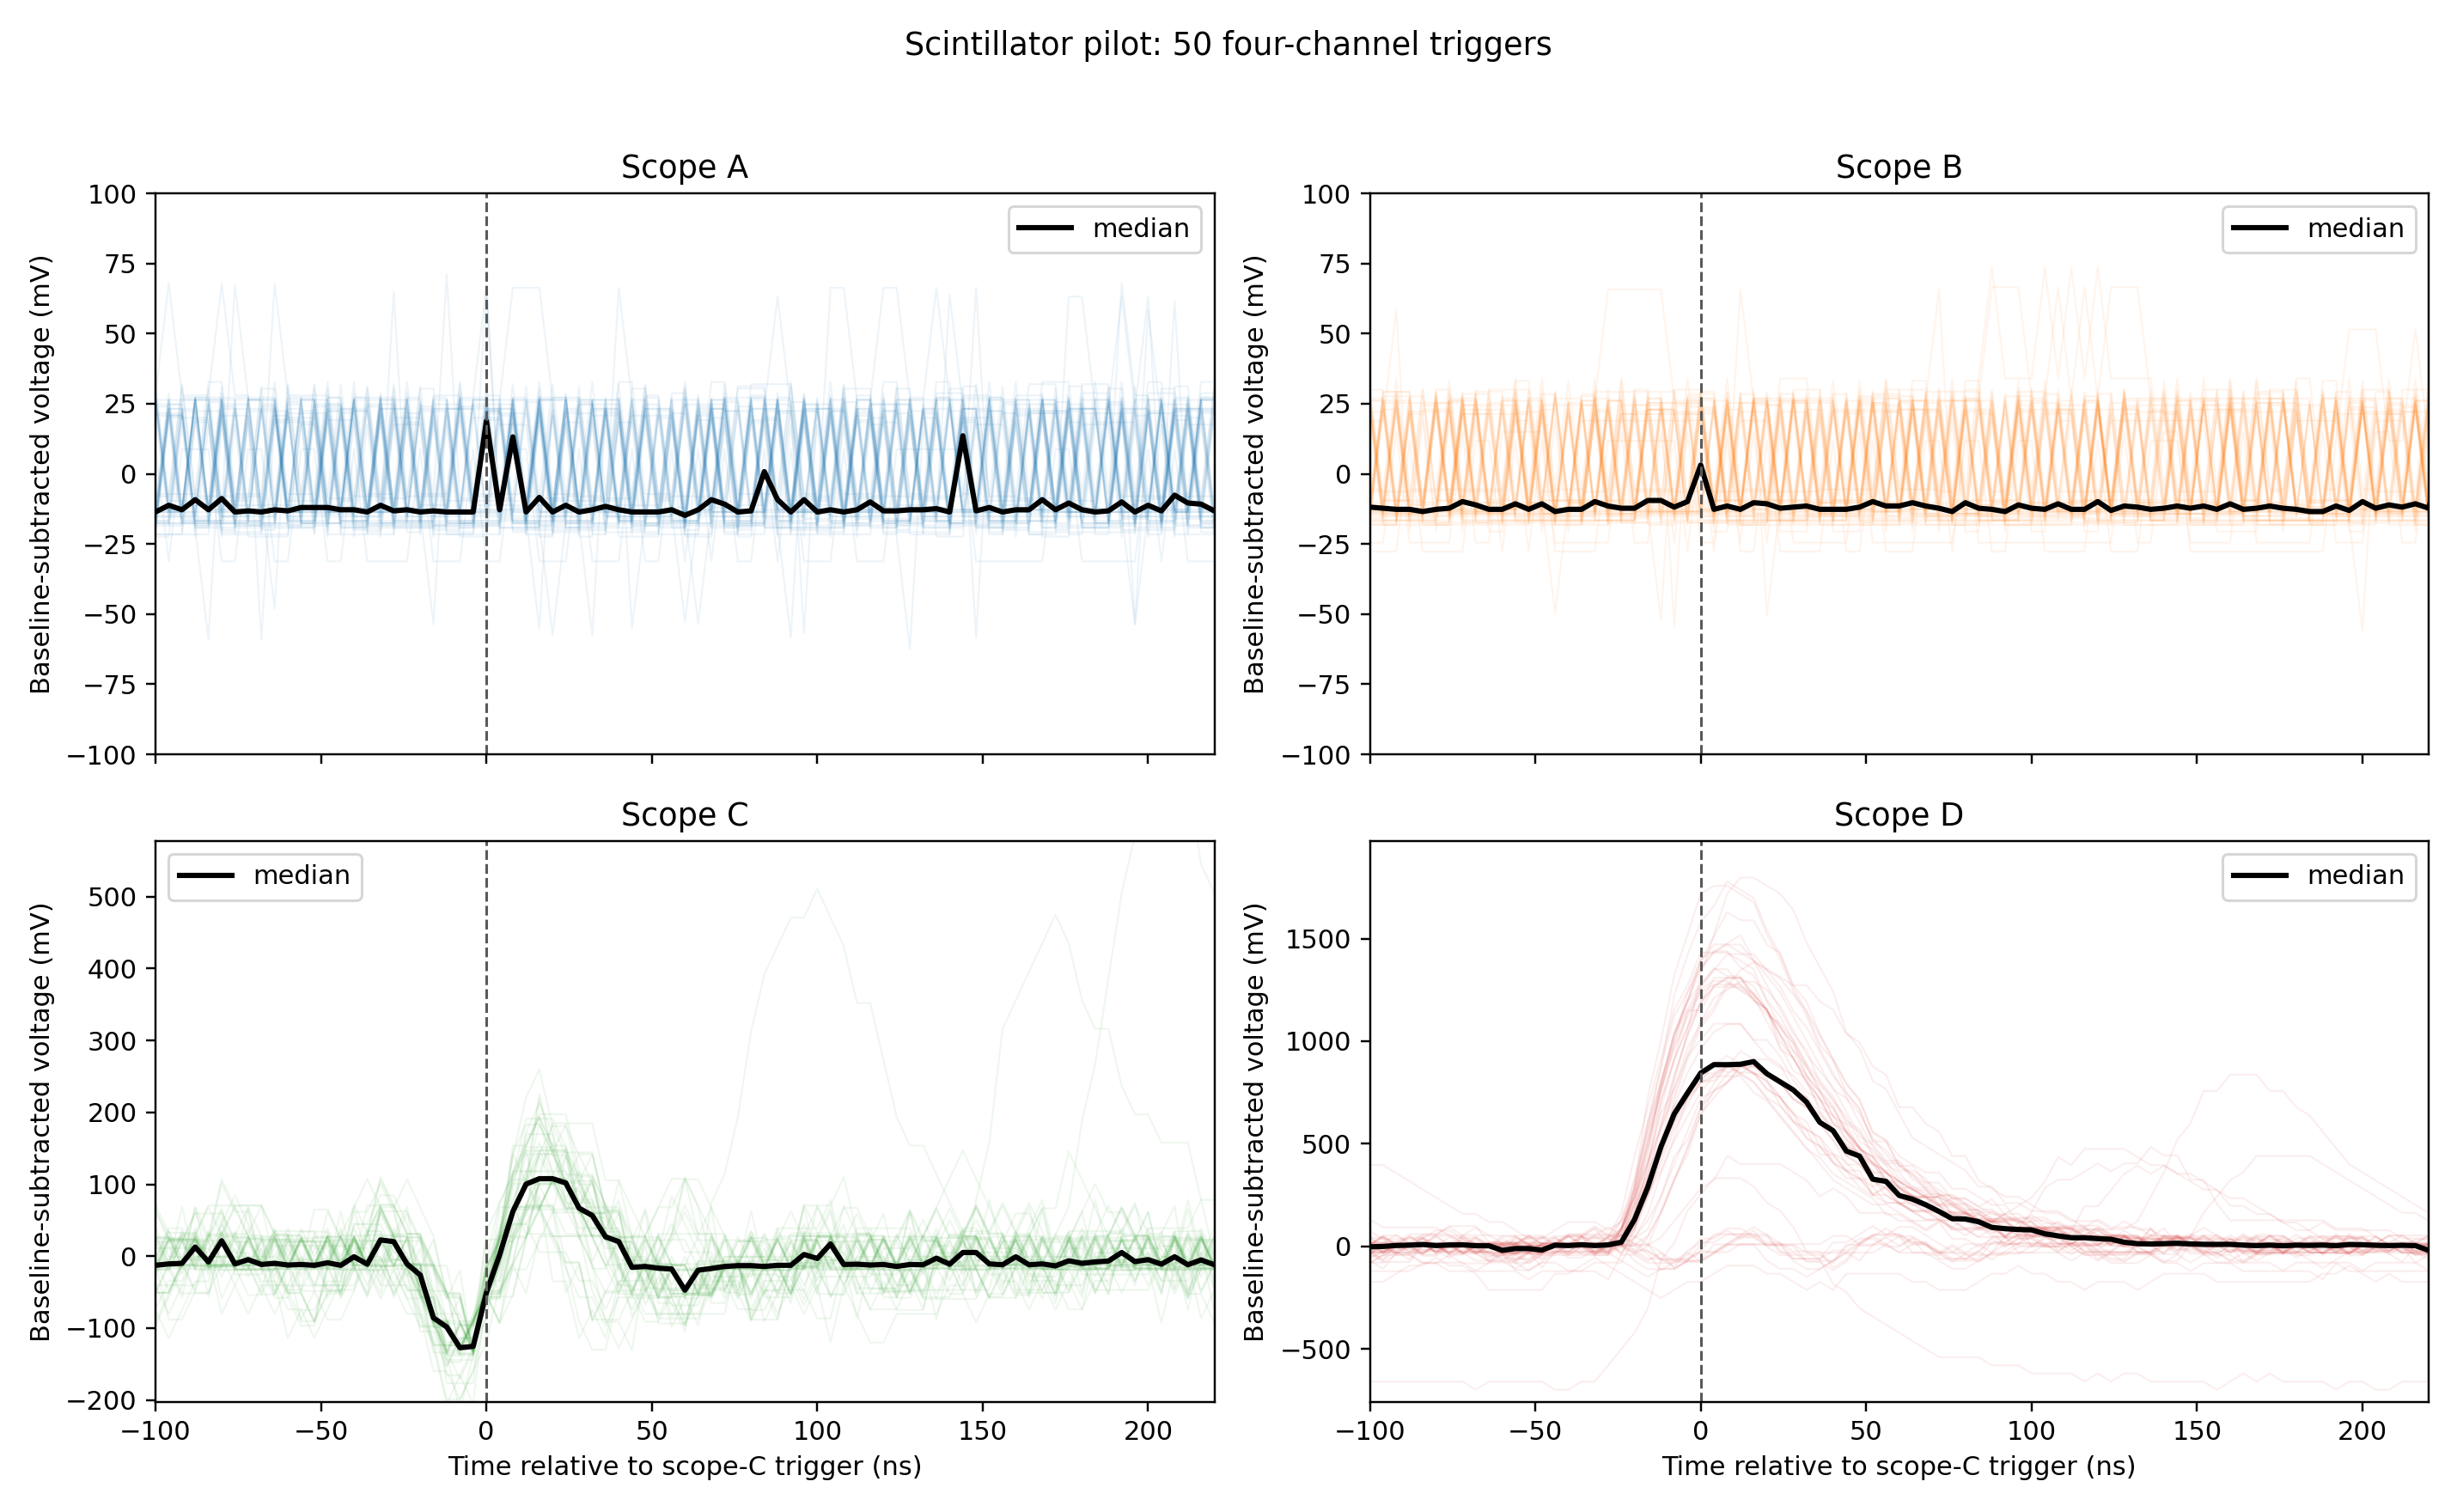
\includegraphics[width=0.98\linewidth]{zero-event-pilot.png}
  \caption{Four-channel waveform pilot for the scintillator zero-event method. The pilot established channel timing and pulse polarity; it was not used as a final efficiency measurement.}
  \label{fig:zero-event-pilot}
\end{figure}

The production configuration requested 1,000 hardware-triggered events, used no auto-trigger, and recorded \SI{4}{\nano\second} sampling over \SI{800}{\nano\second} before and \SI{400}{\nano\second} after the trigger. Reference-channel overflow rejects an event. Saturation on a GSU gLOWCOST channel is retained as an unambiguous hit for the hit-or-miss efficiency measurement, although it cannot be used for pulse-amplitude calibration.

No final efficiency is quoted here. The EPIC SiPM breakdown voltages have not yet been individually measured, and the final reference cuts, accidental contribution, and zero threshold still require validation on a sufficiently large sample.

\section{Discussion}

\subsection{What is established}

The pulse-area method gives internally repeatable breakdown-voltage measurements when several p.e. populations are resolved and trigger acceptance is controlled. This conclusion is supported by independent repeats, interleaved validation points, channel swaps, area-height comparisons, and leave-one-out tests.

The Triangle and Star pair have compatible measured intercepts. Operating them at device-specific $\vbr+\SI{3}{\volt}$ values is more defensible than assigning one common bias without calibration.

The CH3 study also shows why waveform quality and trigger acceptance must be examined before trusting a fit. A small set of biased events can produce a clean line and a high $R^2$. The acceptance transition exposed the problem; $R^2$ alone would not have done so.

\subsection{What is not established}

The quoted internal uncertainties do not include a complete absolute calibration of the delivered SiPM voltage. The MAX1932 relation, channel DAC relation, loading, meter accuracy, and high-minus-low subtraction all contribute to the absolute bias uncertainty.

The measurement also does not yet provide absolute SiPM gain in electrons. The area spacing is in \si{\milli\volt\nano\second} at the amplified scope point. Conversion to charge requires the calibrated transfer impedance and bandwidth of the readout.

Finally, equal overvoltage does not guarantee equal PDE or DCR. PDE depends on wavelength and device properties, while DCR depends strongly on temperature and defects. Optical coupling and tile response enter the complete detector efficiency. The EPIC-triggered measurement and a future pulsed-LED zero-event measurement are therefore necessary parts of operating-point selection.

\subsection{Temperature}

The provisional correction comes from device-family information and uses
$k_T=\SI{54}{\milli\volt\per\degreeCelsius}$. A dedicated controlled-temperature scan is still required for each physical SiPM. At each stable temperature, a shortened p.e.-spacing scan should determine $\vbr(T)$ and fit

\begin{equation}
  \vbr(T)=\vbr(T_0)+k_T(T-T_0).
\end{equation}

The fitted $k_T$ should replace the provisional family value in the detector compensation program. Air temperature alone is not sufficient; the SiPM, PCB, and sensor must reach thermal equilibrium.

\section{Next Measurements}

The following measurements are required before declaring a final operating point:

\begin{enumerate}[leftmargin=*]
  \item Measure the MAX1932 high side and each DAC low side with a calibrated high-impedance meter at several codes. Fit the delivered effective bias and its uncertainty.
  \item Repeat the breakdown-voltage scan at several stable temperatures and measure the individual temperature coefficient of each SiPM.
  \item Complete the EPIC-triggered GSU gLOWCOST zero-event run with enough selected coincidences to measure full-chain efficiency and its statistical interval.
  \item Use a weak, stable pulsed LED near the wavelength-shifting-fibre emission region. Determine the corrected zero fraction at several overvoltages to compare relative photon sensitivity.
  \item Measure dark-count rate, crosstalk, and afterpulsing with an acquisition whose live time and dead time are calibrated.
  \item Verify that the chosen comparator threshold retains the muon-efficiency plateau while suppressing accidental counts.
\end{enumerate}

The final operating point should balance resolved gain, high full-chain efficiency, manageable dark and correlated noise, temperature stability, and margin below analogue saturation. It does not have to be exactly \SI{3}{\volt} overvoltage; that value is the controlled starting point for comparison.

\section{Conclusion}

The existing gLOWCOST analogue readout can resolve photoelectron populations from light-blocked Hamamatsu S13360-2050VE SiPMs. A robust baseline, peak-aligned pulse-area integration, pedestal-constrained p.e. comb, trigger-acceptance check, and repeated gain-versus-bias fit form a practical calibration method.

The original pair showed a substantial device-to-device intercept difference on the present bias scale. The later Triangle and Star pair gave weighted breakdown voltages of \SI{50.512(83)}{\volt} and \SI{50.574(67)}{\volt} near \SI{20.4}{\degreeCelsius}; their difference is not statistically significant. These are internally repeatable operational values, not yet traceable absolute voltages.

The work also identified a readout-path trigger artifact on PCB CH3 and demonstrated that controlling acquisition acceptance is as important as fitting a clean spectrum. The next stage is to calibrate the delivered voltage directly, measure the temperature coefficients, and complete the EPIC-triggered and pulsed-LED zero-event measurements. Those measurements will determine whether equal overvoltage also gives the matched practical sensitivity required for detector operation.

\section*{Acknowledgements}
\addcontentsline{toc}{section}{Acknowledgements}

The detector development and measurements were carried out in the Department of Physics and Astronomy at Georgia State University as part of the gLOWCOST detector program.

\bibliographystyle{unsrt}
\bibliography{references}

\appendix

\section{Software and Reproducibility}

The analysis was performed with Python 3.10, NumPy, pandas, SciPy, and Matplotlib. PicoScope software was used for early manual recordings, and PicoSDK was used for automated acquisition. The main analysis functions used were:

\begin{itemize}[leftmargin=*]
  \item \texttt{numpy.trapezoid} for pulse-area integration;
  \item \texttt{scipy.ndimage.gaussian\_filter1d} for diagnostic histogram smoothing;
  \item \texttt{scipy.signal.find\_peaks} for historical candidate discovery;
  \item \texttt{scipy.optimize.curve\_fit} for historical local Gaussian fits;
  \item \texttt{scipy.optimize.least\_squares} for the simultaneous p.e. comb; and
  \item \texttt{scipy.optimize.brentq} for the additional-scatter solution.
\end{itemize}

The code, compact processed data, figures, and chronological laboratory notes are available at
\url{https://github.com/tharinduudu/SiPM-Operating-Point-Study}. Raw waveform campaigns remain on the acquisition computer because their size is not suitable for Git.

\section{Important Distinction Between Thresholds}

Three different thresholds appear in the study:

\begin{enumerate}[leftmargin=*]
  \item the PicoScope trigger used to decide which waveforms are recorded;
  \item the software boundary used to classify a waveform as zero or nonzero; and
  \item the hardware comparator threshold used by the operating detector.
\end{enumerate}

They have different purposes and must not be interchanged. The \SI{25}{\milli\volt} value used to correct CH3 waveform acquisition is not a recommendation for the normal detector comparator threshold.

\section{Summary of Uncertainty Categories}

\begin{table}[htbp]
  \centering
  \caption{Uncertainty categories and their current treatment.}
  \label{tab:uncertainty-summary}
  \begin{tabularx}{0.94\linewidth}{l Y}
    \toprule
    Source & Treatment \\
    \midrule
    P.e.-spacing statistics & Included in each spectrum-fit uncertainty \\
    Slope-intercept covariance & Included in the internal $\vbr$ uncertainty \\
    Excess point scatter & Added when the observed scatter exceeds point errors \\
    Run-to-run repeatability & Included when compatible independent runs are combined \\
    Absolute high-side calibration & Not yet included \\
    Per-channel DAC calibration & Not yet fully included as a traceable systematic \\
    Temperature coefficient & Provisional family value; individual scan pending \\
    Trigger selection & Tested explicitly; problematic points rejected \\
    Analogue transfer calibration & Not included in absolute charge or gain \\
    \bottomrule
  \end{tabularx}
\end{table}

\end{document}
